%%SUJET MODIFIE POUR LES MP

Drone à géométrie variable
\textit{Inspiré de la thèse de Valentin RIVIERE,
<< Vers un robot aérien autonome bio­inspiré à morphologie variable >>,
Thèse de doctorat en Sciences du Mouvement Humain, Aix-­Marseille, 2019}

\section*{Présentation générale}


Ce sujet porte sur la conception d’un drone quadrirotor bio­inspiré, développé à l’institut des
sciences du mouvement. Ce drone s’inspire de l’oiseau et possède la capacité de se replier
en vol afin de diminuer son envergure (\autoref{fig:01} et \autoref{fig:02}).

En fin de repliement, les bras supportant les moteurs et hélices s’alignent le long du corps
du drone pour éviter que les hélices ne touchent les bords de l’ouverture.

Cette particularité est intéressante pour des problématiques d’évitement d’obstacles dans
des milieux encombrés. Le drone est de plus pourvu d’un algorithme d’estimation de taille
d’obstacles en vol grâce à une perception visuelle monoculaire. Cet algorithme permet de
rendre le drone plus autonome pour éviter les collisions avec son environnement et actionner
son système de changement de forme si cela est nécessaire.

Tout cet ensemble constitue la plateforme Quadmorphing.


\begin{minipage}[c]{.48\linewidth}
\begin{figure}[H]
\centering
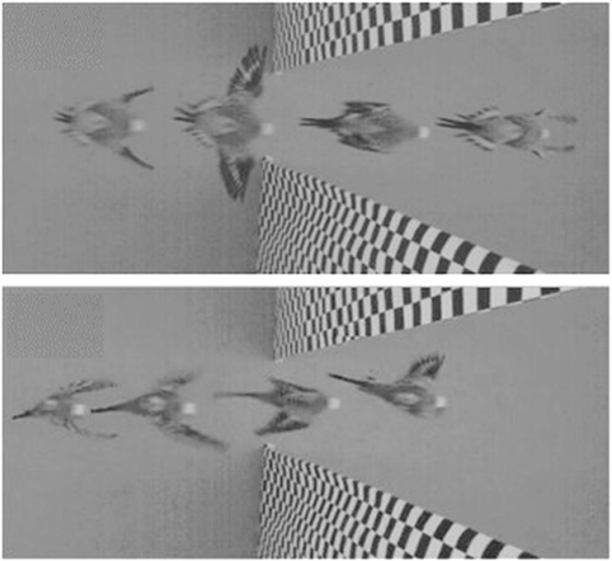
\includegraphics[width=.8\linewidth]{fig_01}
\caption{\label{fig:01} L’oiseau s’adapte au passage
plus étroit en modifiant son envergure}
\end{figure}
\end{minipage}\hfill
\begin{minipage}[c]{.48\linewidth}
\begin{figure}[H]
\centering
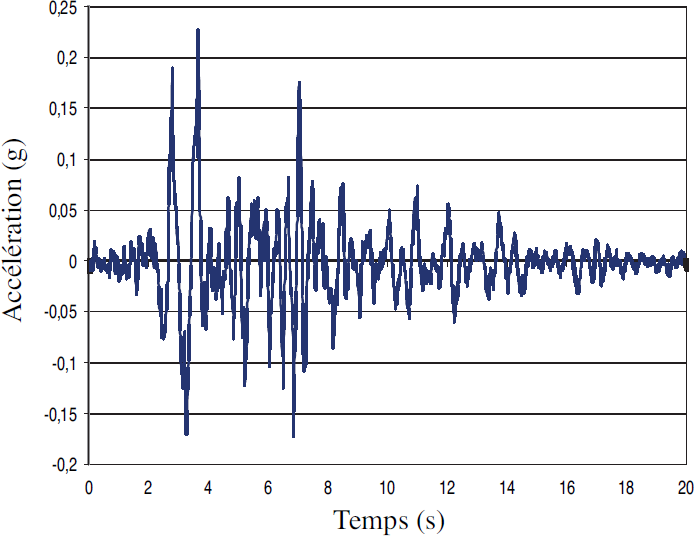
\includegraphics[width=.8\linewidth]{fig_02}
\caption{\label{fig:02} Vue CAO de la plateforme QuadMorphing passant à travers une ouverture}
\end{figure}
\end{minipage}

\begin{obj}
L'objectif de cette étude est de concevoir et valider les solutions technologiques retenues
pour la plateforme QuadMorphing permettant le passage d’ouverture en vol. Le diagramme
partiel des exigences liées à cette étude est donné en \autoref{fig:21} de l’annexe 1.
La démarche proposée est définie ci­-après :
\begin{itemize}
\item ­\autoref{sec:01} --­ influence des mouvements des bras du drone sur son comportement;
\item ­\autoref{sec:02} --­ choix d’un mécanisme de modification de l’envergure;
\item ­\autoref{sec:03} --­ analyse simplifiée de l’asservissement en roulis du drone.
\end{itemize}
\end{obj}

\section{\label{sec:01} Influence des mouvements des bras du drone sur son comportement}

Indépendamment de la solution retenue pour mettre en mouvement les bras supportant les
moteurs et hélices, nous nous intéressons dans cette partie aux conséquences des mouvements des bras sur le comportement dynamique du drone afin de valider les choix retenus
par la suite.

\subsection{Influence de la rotation des bras sur l’envergure ­ vérification des exigences Id 1
et Id 1.1}

Pour diminuer l’envergure, on choisit de replier les bras supportant les moteurs et hélices du
drone. Le repliement doit être rapide et de courte durée. En effet, pour des raisons de contrôle
et de stabilité, il est impossible d’utiliser un drone avec les bras repliés en permanence. La
\autoref{fig:23} de l’annexe 2 présente un modèle géométrique simplifié du drone pour lequel le
bras \textbf{1}, supportant les deux moteurs et hélices avant, peut tourner par rapport au corps \textbf{0} du
drone. Le bras \textbf{2}, supportant les deux moteurs et hélices arrière, peut également tourner par
rapport au corps \textbf{0}. Aussi pour cette étude d’envergure, l’analyse portera sur le bras \textbf{1} seul,
le comportement du bras \textbf{2} étant identique. La \autoref{fig:23} précise le paramétrage associé à
cette étude. L’angle de rotation du bras \textbf{1} par rapport au corps \textbf{0} du drone est noté $\gamma_1$ et peut
atteindre n’importe quelle valeur dans l’intervalle $[0\degres, 90\degres]$.
L’angle de rotation du bras \textbf{2} par rapport au corps \textbf{0} du drone est noté $\gamma_2$ et peut atteindre
n’importe quelle valeur dans l’intervalle $[90\degres, 180\degres]$.

%Q01
\question{\label{q:01} À partir de la \autoref{fig:23} de l’annexe 2, déterminer l’expression de la largeur $\ell$ en fonction de $\gamma_1$ et des données de la géométrie du drone.}
\ifprof
\begin{corrige}
\end{corrige}
\else
\fi

%Q02
\question{\label{q:02} En déduire la valeur de la réduction d’envergure $A =  1 - \dfrac{\indice{\ell}{min}}{\indice{\ell}{max}}$ et l’exprimer en \%.
Conclure sur la performance liée à l’exigence de réduction d’envergure Id 1.1.}
\ifprof
\begin{corrige}
\end{corrige}
\else
\fi


Des essais expérimentaux ont été réalisés pour analyser le passage du drone au travers
d’une ouverture carrée de taille de $\SI{20}{cm} \times \SI{20}{cm}$ et de profondeur de $\SI{1}{cm}$. L’ouverture est placée verticalement par rapport au sol et un de ses côtés est orienté horizontalement
(parallèle au sol). Selon la \autoref{fig:02}, le repère $\rep{G}$ est associé à cette ouverture 
(origine $\vect{O_G}$ centrée par rapport à l’ouverture). Pour la suite, la position 
$\vect{O_G O} = x_G \vect{x_G}+y_G \vect{y_G}+z_G \vect{z_G}$
 correspond à la position du centre d’inertie $O$ du drone par rapport au repère $\rep{G}$.

On définit selon la \autoref{fig:03} et la \autoref{fig:04}, la longueur projetée $\indice{\ell}{proj}$ et la hauteur projetée $\indice{h}{proj}$ du
drone dans le plan de l’ouverture. Les bords avant gauche et arrière droit du drone sont
représentés respectivement par les points $\indice{\ell}{gauche}$ et $\indice{\ell}{droit}$. Les bords avant haut et arrière bas
du drone sont représentés respectivement par les points $\indice{h}{haut}$ et $\indice{h}{bas}$.
Ces grandeurs dépendent des dimensions du drone et de son orientation par rapport à $\rep{G}$. En
première approximation et en considérant un angle de roulis $\indice{\theta}{R}$ (rotation autour de $\axe{O}{x_0}$) nul
lors du passage de l’obstacle, la longueur projetée $\indice{\ell}{proj}$ dépend uniquement des dimensions
du drone et de l’angle de lacet $\indice{\theta}{L}$ (rotation autour de $\axe{O}{z_0}$), et la hauteur projetée $\indice{h}{proj}$ dépend
uniquement des dimensions du drone et de l’angle de tangage $\indice{\theta}{T}$ (rotation autour de $\axe{O}{y_0}$).


\noindent
\begin{minipage}[c]{.48\linewidth}
\begin{figure}[H]
\centering
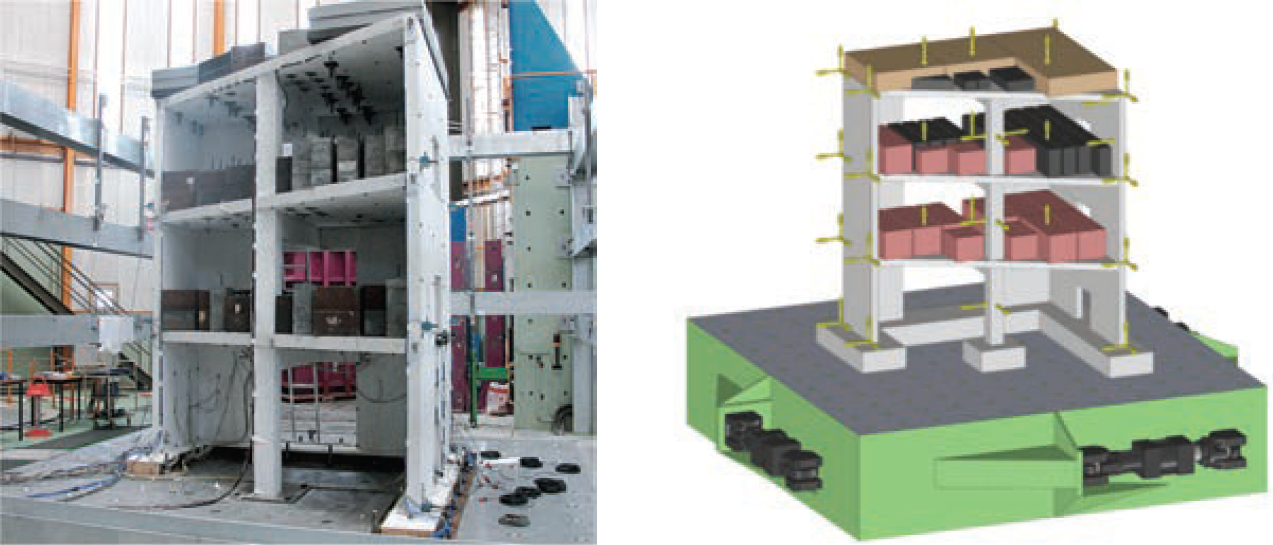
\includegraphics[width=\linewidth]{fig_03}
\caption{\label{fig:03} ­Définition de la longueur projetée $\indice{\ell}{proj}$ et de l’angle de lacet $\indice{\theta}{L}$}
\end{figure}
\end{minipage}\hspace{.5cm}
\begin{minipage}[c]{.48\linewidth}
\begin{figure}[H]
\centering
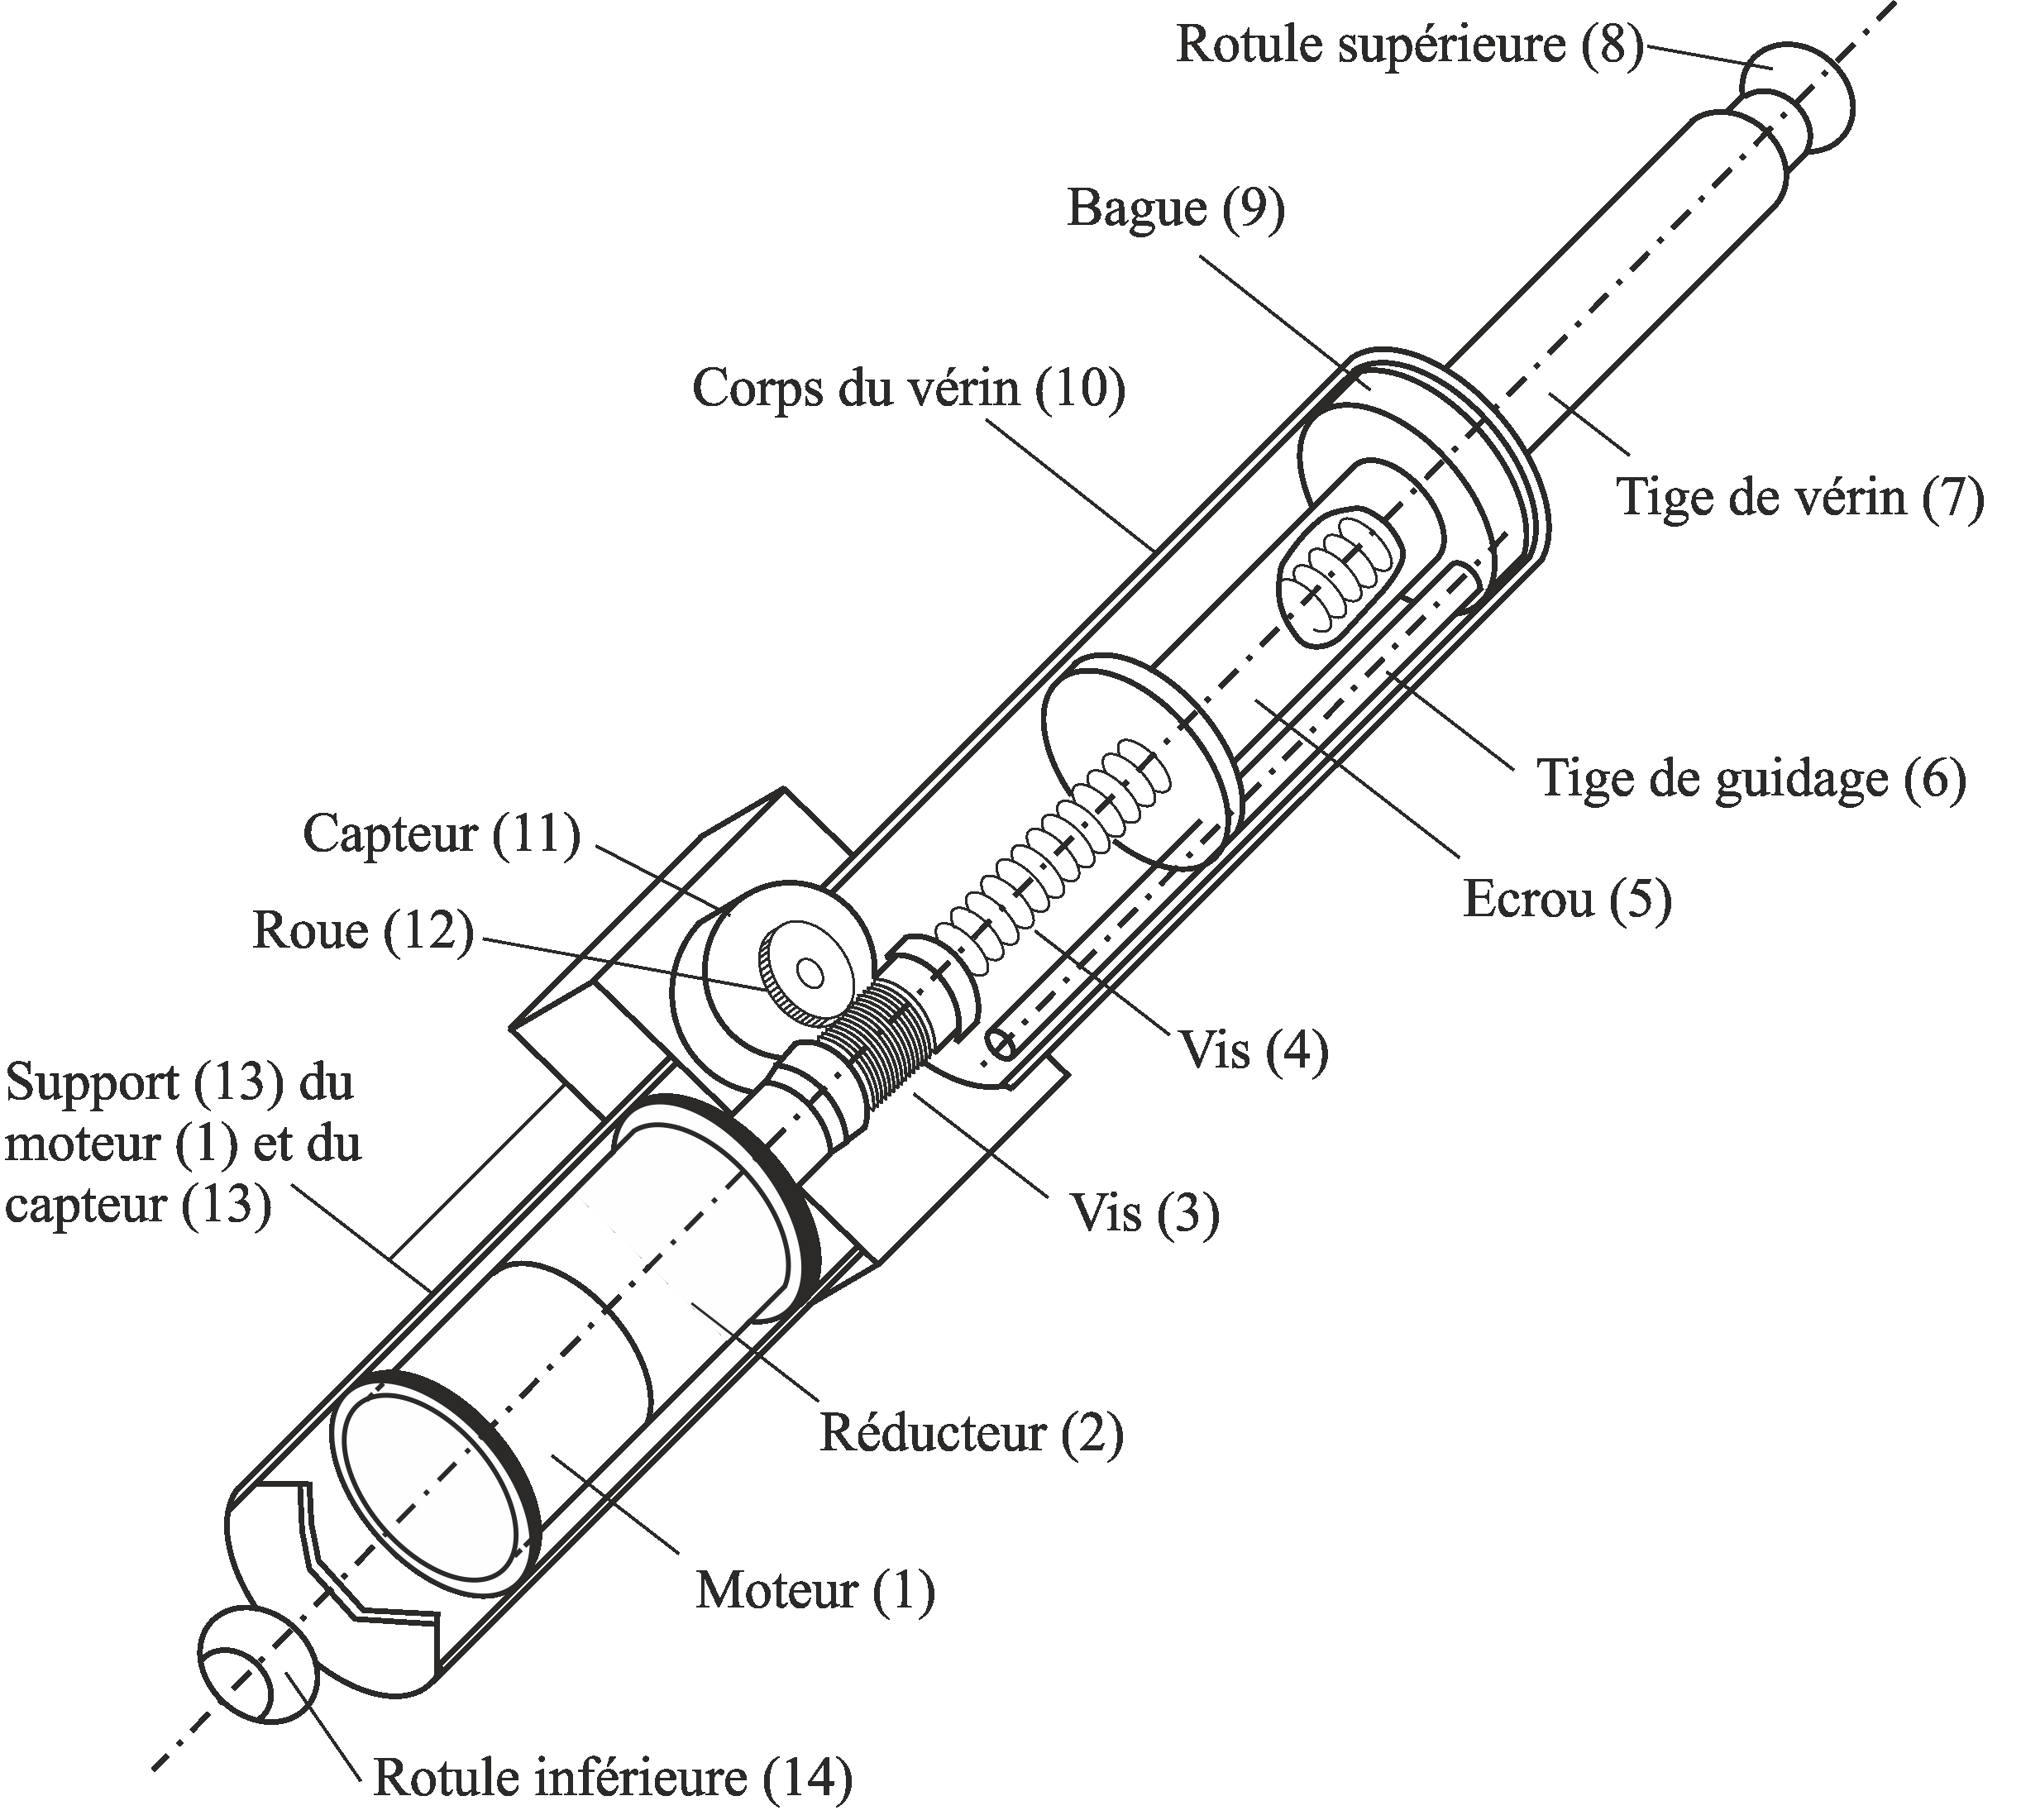
\includegraphics[width=\linewidth]{fig_04}
\caption{\label{fig:04} ­Définition de la longueur projetée $\indice{h}{proj}$ et de l’angle de lacet $\indice{\theta}{T}$}
\end{figure}
\end{minipage}

\vspace{.25cm}

Les relevés expérimentaux de 8 essais avec manœuvre de repliement des bras et passage de l’ouverture sont donnés en \autoref{fig:05}. La zone hachurée représente l’envergure de l’ouverture durant toutes les positions du robot où les collisions sont possibles, c’est­-à-­dire pour $x_G \in \left[-L/2, L/2 \right]$. L’aire grisée représente l’envergure maximale occupée par le drone durant les huit essais. Les positions des points extrêmes du drone de l’essai n°4 ($\indice{\ell}{gauche}$, $\indice{\ell}{droit}$, $\indice{h}{haut}$ et $\indice{h}{bas}$) sont représentées par les courbes avec le marqueur en forme de losange $\Diamond$. On
peut observer sur ces figures la diminution de l’envergure horizontale du drone à partir de la
consigne de repliement (représentée verticalement en pointillés à gauche). La consigne de
dépliement de la structure (représentée verticalement en pointillés à droite) est donnée dès
la sortie de la zone probable de collision afin de stabiliser le drone au plus vite.

\begin{figure}[H]
\centering
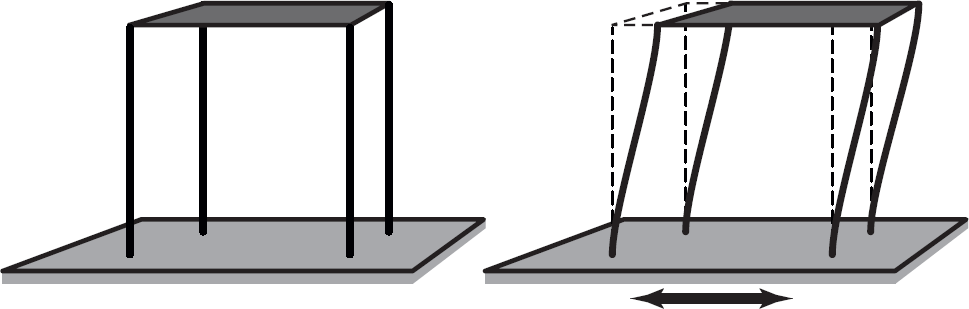
\includegraphics[width=\linewidth]{fig_05}
\caption{\label{fig:05} Vues de dessus et de côté de l’envergure du drone durant huitpassages de l’ouverture}
\end{figure}


%Q03
\question{\label{q:03}  Relever pour l’essai n°4, la valeur de $\indice{\ell}{proj}$ avant repliement (notée $\indice{\ell}{proj}^{\text{max}}$) et la comparer
à $\indice{\ell}{max}$ de la question précédente. De même pour la valeur après repliement (notée
$\indice{\ell}{proj}^{\text{min}}$) à comparer à $\indice{\ell}{min}$.
Si des écarts sont constatés entre les valeurs expérimentales et les valeurs théoriques,
expliquer l’(les) origine(s) de ces écarts.
Conclure sur la vérification de l’exigence liée au passage d’ouverture Id 1.}
\ifprof
\begin{corrige}
\end{corrige}
\else
\fi

\subsection{Influence de la rotation des bras sur la vitesse maximale en bout de pale ­-- Vérification de l’exigence Id 4}

On considère que le drone se déplace en ligne droite à la vitesse de déplacement $V_x\vect{x_0}$
selon $\vect{x_0} = \vect{x_G}$ telle que $V_x = \SI{2,5}{m.s^{-1}}$. Cette vitesse correspond à la vitesse retenue pour négocier
le passage de l’ouverture. Elle est suffisamment lente pour que le drone ait le temps d’interpréter la taille de l’ouverture et de décider si elle est franchissable ou non (dans ce cas
le drone doit avoir le temps de réaliser un freinage d’urgence avant collision). Par ailleurs,
cette vitesse est suffisamment rapide pour conserver un minimum <<~d’inertie~>> lors du franchissement et permettre sa stabilisation une fois l’ouverture franchie et les bras dépliés.

La \autoref{fig:23} et la \autoref{fig:24} complètent le paramétrage. 
On suppose que le référentiel terrestre
associé à $\rep{G}$ peut être considéré galiléen. On pose de plus $\alpha = \angl{x_1}{\indice{x}{H1}}$ l’angle définissant
l’orientation de l’hélice \textbf{H1} par rapport au bras \textbf{1}.

La vitesse de rotation du bras \textbf{1} par rapport au corps \textbf{0} du drone, $\vecto{1}{\rep{0}}$, est telle que $\vecto{1}{\rep{0}} = \dot{\gamma}_1\vz{0}$. La valeur maximale de cette vitesse est obtenue par une rotation de 90\degres en \SI{300}{ms}.
La vitesse de rotation de l’hélice \textbf{H1} par rapport au bras \textbf{1}, $\vecto{H1}{\rep{1}}$, est telle que 
$\vecto{H1}{\rep{1}} = \omega_1\vz{0} = \alphap \vz{0}$. 
On considérera que la vitesse de rotation de l’hélice est égale à
\SI{13 400}{tr/min} pour assurer la portance et le déplacement horizontal du drone à $V_x = \SI{2,5}{m.s^{-1}}$.

%Q04
\question{\label{q:04} Déterminer l’expression littérale de $\vectv{P}{H1}{\rep{G}}$, la vitesse en bout de pale de l’hélice
\textbf{H1} par rapport à $\rep{G}$, en fonction des données et notamment de $\dot{\gamma}$ et de $\omega_1$.}
\ifprof
\begin{corrige}
\end{corrige}
\else
\fi

%Q05
\question{\label{q:05} Dans quelle configuration du bras et de la pale cette vitesse en bout de pale est­elle
maximale ?
Déterminer dans ce cas l’expression maximale de la norme, notée $\indice{V}{max}$. Réaliser l’application numérique en déterminant au préalable la valeur numérique de chacun des
termes de l’expression de $\indice{V}{max}$.
Commenter l’influence de la vitesse de rotation des bras du drone sur la valeur de
$\indice{V}{max}$ et sur la vérification de l’exigence Id 4}
\ifprof
\begin{corrige}
\end{corrige}
\else
\fi

\subsection{Influence de la rotation des bras sur le comportement dynamique du drone selon
l’axe de lacet ­ vérification de l’exigence Id 1.1.1}

On cherche à déterminer la relation à donner entre les rotations $\gamma_1$ et $\gamma_2$ des deux bras du
drone de manière à limiter les perturbations sur le comportement dynamique en vol du drone
lors des phases de repliement et dépliement. L’objectif est d’avoir un moment dynamique du
drone selon l’axe de lacet (axe $\axe{O}{z_0}$) en $O$, centre d’inertie du drone, indépendant de $\gamma_1$
et $\gamma_2$ (et de leurs dérivées successives). Les matrices d’inerties des principaux éléments du
drone, dont la géométrie a été simplifiée pour cette étude, sont données en annexe 3.

\begin{hypo}
On suppose le drone en vol rectiligne à vitesse constante et à altitude constante. Le référentiel associé au repère $\rep{0}$ lié au corps du drone peut être considéré galiléen.
Les vitesses de rotation des hélices sont telles que :
\begin{itemize}
\item $|\omega_1|=|\omega_2|=\omega$ constante,
\item $|\omega_3|=|\omega_4|=\omega'$ constante.
\end{itemize}
Les bras sont en phase de repliement ou dépliement, 
donc $\gamma_1 \in ]0\degres, 90\degres]$, 
$\dot{\gamma}_1 \neq 0$ et  $\ddot{\gamma}_1 \neq 0$ pour le bras \textbf{1};
idem pour les dérivées de l’angle $\gamma_2$ du bras \textbf{2}.
\end{hypo}



%Q06
\question{\label{q:06}Déterminer l’expression littérale du moment dynamique du bras \textbf{1} calculé en $O$ selon $\vz{0}$ : $\vectmd{O}{1}{\rep{0}}\cdot \vz{0}$. En déduire l’expression littérale du moment dynamique du bras \textbf{2}
calculé en $O$ selon $\vz{0}$ : $\vectmd{O}{2}{\rep{0}}\cdot \vz{0}$.}
\ifprof
\begin{corrige}
\end{corrige}
\else
\fi


%Q07
\question{\label{q:07} Déterminer l’expression littérale du moment dynamique de l'hélice \textbf{H1} calculé en $O$ selon $\vz{0}$ : $\vectmd{O}{H1}{\rep{0}}\cdot \vz{0}$.}
\ifprof
\begin{corrige}
\end{corrige}
\else
\fi


%Q08
\question{\label{q:08} En déduire l’expression littérale du moment dynamique de l'hélice \textbf{H2} calculé en $O$ selon $\vz{0}$ : $\vectmd{O}{H2}{\rep{0}}\cdot \vz{0}$.}
\ifprof
\begin{corrige}
\end{corrige}
\else
\fi


On donne pour la suite l’expression littérale du moment dynamique de l’ensemble hélice \textbf{H3}
+ hélice \textbf{H4} calculé en $O$ selon $\vz{0}$ : $\vectmd{O}{H3+H4}{\rep{0}} \cdot \vz{0} = 2 I_{hz} \ddot{\gamma}_2 + 2m_h \left(\dfrac{L_1}{2}\right)^2 \ddot{\gamma}_2$.

%Q09
\question{\label{q:09} À partir des résultats des trois questions précédentes, montrer que l’expression du
moment dynamique de l’ensemble $\Sigma$, calculé en $O$ selon $\vz{0}$, se met sous la forme  :
$\vectmd{O}{\Sigma}{\rep{0}}\cdot \vz{0} = 2 \indice{I}{eq} \left(\gammapp_1+\gammapp_2\right)$ 
où $\indice{I}{eq}$ est une constante dont l’expression est à préciser.}
\ifprof
\begin{corrige}

\end{corrige}
\else
\fi

La commande retenue pour le repliement et dépliement des bras du drone satisfait la relation
suivante : $\gamma_2 = \pi - \gamma_1$.


%Q10
\question{\label{q:10}Expliquer en quoi ce choix de conception permet de vérifier l’exigence Id 1.1.1.}
\ifprof
\begin{corrige}
\end{corrige}
\else
\fi



\subsection{Influence de la rotation des bras sur l’inertie du drone ­ analyse de l’exigence Id 1.2}
On se propose de déterminer les variations, dues à la rotation des bras, de la matrice d’inertie
totale du drone en $O$ exprimée dans la base $\base{x_0}{y_0}{z_0}$. On considère pour ceci une géométrie
simplifiée du drone (\autoref{fig:06}) composée du châssis intégrant la caméra et la batterie, des
deux bras et des 4 sous­ensembles \{moteurs brushless + hélice\} modélisés par des masses
ponctuelles, de masse $m_E = \indice{m}{moteur}+m_h$ (dans cette sous­partie les inerties des axes moteurs
et hélices sont négligées devant les autres grandeurs). On rappelle que $\gamma_2 = \pi - \gamma_1$.
En additionnant les matrices d’inertie du corps \textbf{0}, du drone et des bras \textbf{1} et \textbf{2} exprimées en $O$
dans la base $\bas{0}$, l’inertie de l’ensemble, en tenant compte également des moteurs brushless
et des hélices, se met sous la forme : $\inertie{O}{\Sigma} = \matinertie{I_{\Sigma X}}{I_{\Sigma Y}}{I_{\Sigma Z}}{I_{\Sigma yz}}{I_{\Sigma xz}}{I_{\Sigma xy}}{O,\bas{0}}$
où les termes $I_{\Sigma X}$, $I_{\Sigma Y}$ sont des fonctions de $\gamma_1$ et de la géométrie et $I_{\Sigma Z}$ est uniquement
fonction de la géométrie (et donc indépendant de $\gamma_1$).

%Q11
\question{\label{q:11} Compte tenu de la géométrie retenue, simplifier la forme de la matrice d’inertie totale  $\inertie{O}{\Sigma}$. Justifier vos simplifications.}
\ifprof
\begin{corrige}

\end{corrige}
\else
\fi


La relation entre $\gamma_1$ et $\gamma_2$ permet finalement d’avoir une matrice d’inertie de l’ensemble du
drone qui est quasiment diagonale pour toutes valeurs de $\gamma_1$, ce qui évite le couplage des
équations de roulis, tangage et lacet et facilite ainsi le contrôle du drone. Cela permet également d’avoir un moment d’inertie selon l’axe de lacet  $I_{\Sigma Z}$ indépendant de la position des
bras.

\begin{figure}[H]
\centering
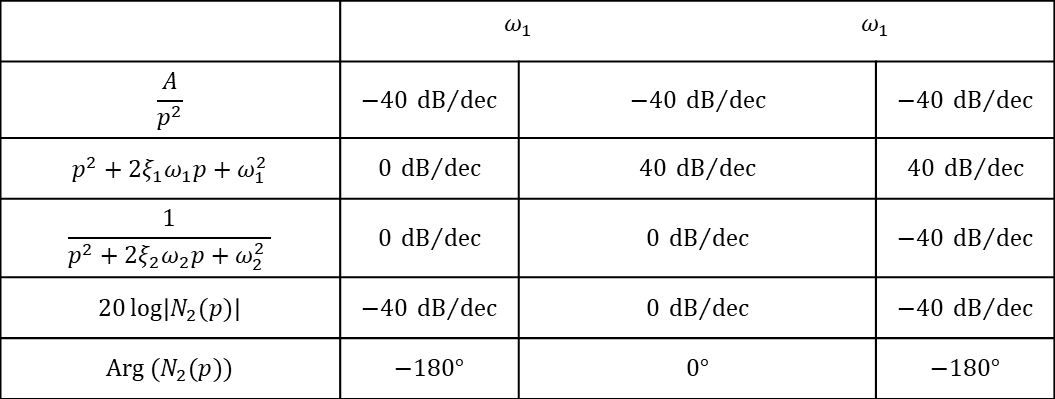
\includegraphics[width=.8\linewidth]{fig_06}
\caption{\label{fig:06}  Figure simplifiée de la géométrie du drone}
\end{figure}

On note pour la suite $\Delta I_{\Sigma Z} (\gamma_1)$ et $\Delta I_{\Sigma Y} (\gamma_1)$  les variations d’inertie en roulis, respectivement en tangage, fonctions de $\gamma_1$, 
telles que : $I_{\Sigma X} = \Delta I_{\Sigma X} (\gamma_1) + I_{\Sigma X}^{\text{cte}}$ 
et 
$I_{\Sigma Y} = \Delta I_{\Sigma Y} (\gamma_1) + I_{\Sigma Y}^{\text{cte}}$ 
où $I_{\Sigma X}^{\text{cte}}$ et $I_{\Sigma Y}^{\text{cte}}$
représentent les termes constants des moments d’inertie indépendants de $\gamma_1$.


\begin{figure}[H]
\centering
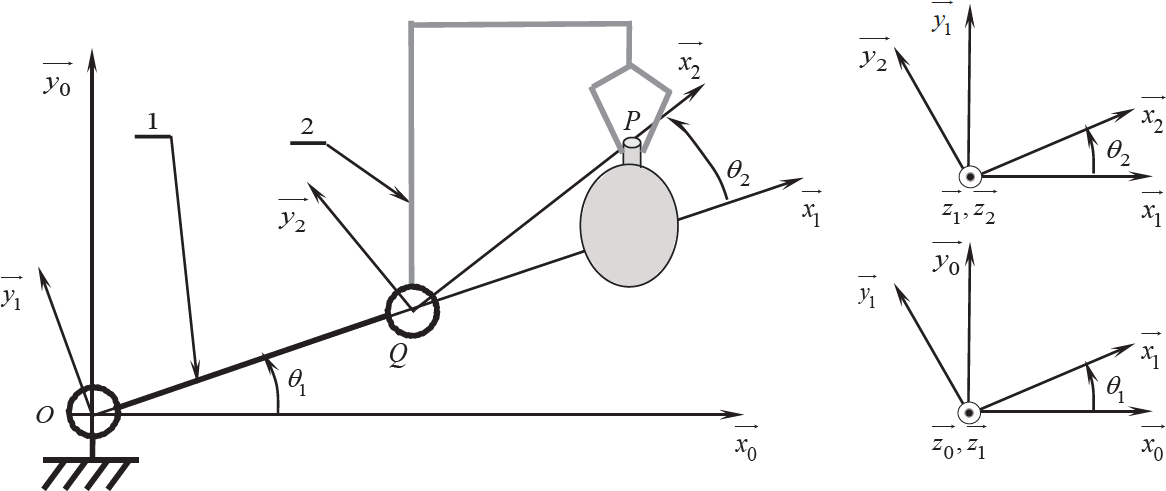
\includegraphics[width=.7\linewidth]{fig_07}
\caption{\label{fig:07}  Évolution de $\Delta I_{\Sigma X}$ et de $\Delta I_{\Sigma Y}$ en fonction de $\gamma_1$. Les bras sont dépliés pour $\gamma_1 = 90\degres$
et pliés (c’est-­-à­dire alignés avec le corps du drone) pour $\gamma_1 = 0\degres$}
\end{figure}

Les évolutions de $\Delta I_{\Sigma X} (\gamma_1)$ et de $\Delta I_{\Sigma Y} (\gamma_1)$ en fonction de $\gamma_1$ sont données \autoref{fig:07}. On donne
de plus ci-­dessous les valeurs numériques, en \si{kg.m^2}, de la matrice d’inertie de la géométrie
simplifiée du drone pour la position bras dépliés ($\gamma_1 = 90\degres$) :
$\inertie{O}{\Sigma}_{\gamma_1 = 90\degres} = \matinertie{\num{5,3e-4}}{\num{1,96e-3}}{\num{1,72e-3}}{0}{0}{0}{O,\bas{0}}$.

%Q12
\question{\label{q:12} En déduire, en \%, les variations maximales d’inertie en roulis, définie par 
$\dfrac{\Delta I_{\Sigma X}}{I_{\Sigma X}\left(\gamma_1 = 90\degres\right)}$
et en tangage, définie par 
$\dfrac{\Delta I_{\Sigma Y}}{I_{\Sigma Y}\left(\gamma_1 = 90\degres\right)}$. Conclure sur la différence de comportement
en vol du drone en roulis et en tangage une fois les bras pliés.}
\ifprof
\begin{corrige}
\end{corrige}
\else
\fi

\subsection{Influence du sens de rotation des hélices sur le comportement dynamique du
drone ­ analyse de l’exigence Id 1.2}

Le fait d’entraîner en rotation une pale d’hélice à la vitesse de rotation $\omega_i$ crée une vitesse
relative entre la pale et l’air. Ce phénomène génère ainsi un effort élémentaire $\vect{\dd F}$ qui peut
être projeté (\autoref{fig:08}) sur l’axe de rotation (composante $\vect{\dd P}$) et dans le plan de rotation (composante $\vect{\dd T}$).
En sommant ces efforts sur un tour d’hélice et en intégrant sur toute la longueur de la pale,
il en résulte une force résultante $\vect{T}$, perpendiculaire au plan de rotation (la poussée), ainsi
qu’un moment résultant $\vect{Q}$ s’exerçant à l’opposé du sens de rotation (le couple de traînée).


\begin{figure}[H]
\centering
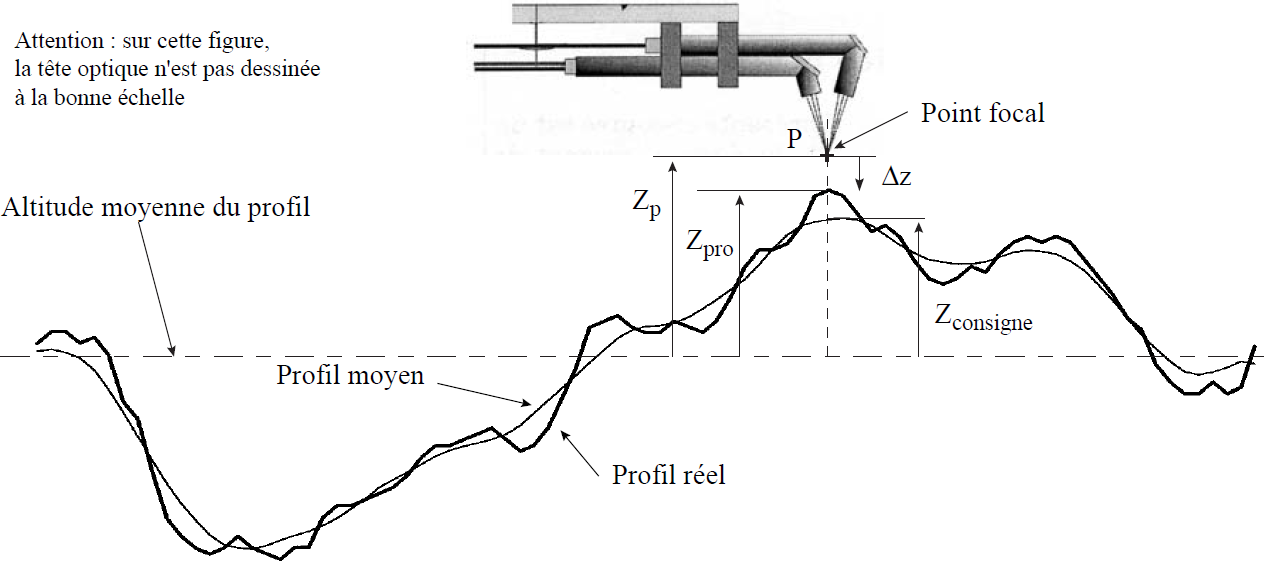
\includegraphics[width=.7\linewidth]{fig_08}
\caption{\label{fig:08}  Représentation de l’action élémentaire de l’air sur une section de pale et de ses
projections lors de sa rotation}
\end{figure}

L’action mécanique de l’air sur l’hélice H1 peut donc être modélisée par l’action mécanique
résultante suivante, pour une rotation du rotor dans le sens positif : 
$\torseurstat{T}{\text{Air}}{H1} = \torseurl{\vect{T}=T\vect{z_0}}{\vect{Q}=-Q\vect{z_0}}{I_1}$
avec $T = c_T \omega_i^2$ et $Q=c_Q \omega_i^2$.


Ces actions, retrouvées au niveau de chacune des hélices, permettent de générer les forces
et moments s’exerçant sur le drone en vue de son contrôle.

Afin de limiter l’influence des moments de traînée de chaque hélice sur le comportement
dynamique du drone en vol stationnaire (cas où les hélices tournent toutes à la même vitesse
et génèrent une poussée résultante compensant le poids du drone), on souhaite déterminer
le sens de rotation de chacun des rotors


\begin{hypo}
On suppose que, quel que soit le sens de rotation du rotor, la portance s’oppose toujours à
l’action du poids (les hélices sont choisies dans ce but).
\end{hypo}

%Q13
\question{\label{q:13} Sur la figure du DR, représenter les actions mécaniques $\vect{T}$ et $\vect{Q}$ pour chacune des
hélices (en trait plein pour les résultantes et en pointillés pour les moments).
En déduire si le drone est à l’équilibre ou non.}
\ifprof
\begin{corrige}
\end{corrige}
\else
\fi

Pour la suite, les hélices génèrent une poussée résultante compensant le poids du drone.
Les sens des vitesses de rotation des hélices s’opposent deux à deux selon la représentation
de la \autoref{fig:09} et ce qu’elle que soit la position des bras. Les hélices \textbf{H1} et \textbf{H3} tournent dans
le sens trigonométrique et les hélices \textbf{H2} et \textbf{H4} dans le sens horaire.

\begin{figure}[H]
\centering
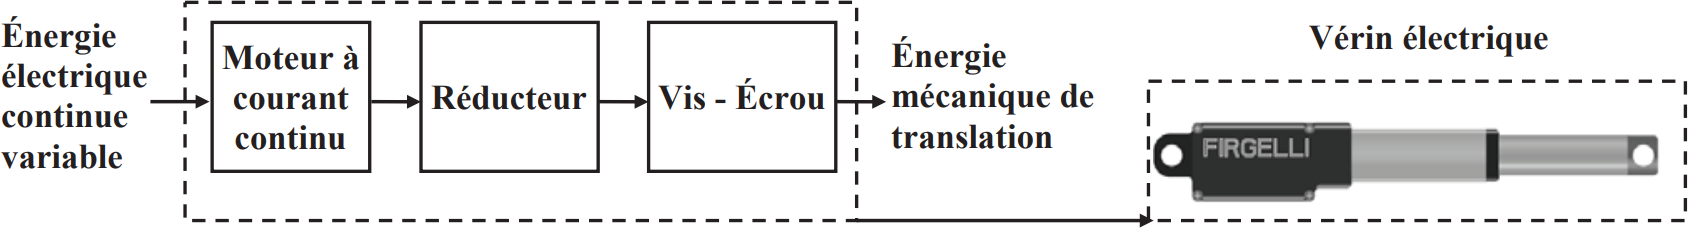
\includegraphics[width=.8\linewidth]{fig_09}
\caption{\label{fig:09} ­Sens de rotation des hélices du drone}
\end{figure}

%Q14
\question{\label{q:14} Quel est alors le comportement du drone dans le cas où $|\omega_1| = |\omega_2|$ et $|\omega_3| = |\omega_4|$ avec
$|\omega_1| < |\omega_3|$ ?
Vous pouvez vous aider d’un schéma pour représenter les actions et justifier votre
réponse.}
\ifprof
\begin{corrige}

\end{corrige}
\else
\fi
Pour la question suivante, on considérera que les hélices tournent toutes à la même vitesse
et génèrent une poussée résultante compensant le poids du drone.

%Q15
\question{\label{q:15} Déterminer l’expression du torseur de l’action de l’air sur l’hélice H1 (défini par l’équation (1)) calculé au point $O$, centre d’inertie du drone. Les composantes du torseur
seront données dans la base $\bas{0}$ en fonction des grandeurs géométriques, de $\gamma_1$, de
$c_T$, $c_Q$ et de $\omega_1$.}
\ifprof
\begin{corrige}
\end{corrige}
\else
\fi

On donne pour la suite la matrice $\Gamma (\gamma_1)$ permettant de relier les carrés des vitesses de rotation
des hélices à la poussée résultante et aux moments résultants exprimés en $O$ selon les axes
du drone (respectivement roulis selon $\vx{0}$, tangage selon $\vy{0}$ et lacet selon $\vz{0}$).

$$
\begin{pmatrix}
\sum\limits_{i=1}^{4} \vectf{\text{air}}{H_i} \cdot\vz{0} \\
\sum\limits_{i=1}^{4} \vectm{O}{\text{air}}{H_i} \cdot\vx{0} \\
\sum\limits_{i=1}^{4} \vectm{O}{\text{air}}{H_i} \cdot\vy{0} \\
\sum\limits_{i=1}^{4} \vectm{O}{\text{air}}{H_i} \cdot\vz{0} 
\end{pmatrix}
=
\underbrace{\begin{pmatrix}
\cdots & c_T & C_T & c_T  \\
\cdots & c_t \dfrac{L_1}{2} \sin \gamma_1 & c_t \dfrac{L_1}{2} \sin \gamma_1 & - c_t \dfrac{L_1}{2} \sin \gamma_1 \\
\cdots 
& - \left(\dfrac{L_0}{2} + \dfrac{L_1}{2} \cos \gamma_1 \right) 
& \left(\dfrac{L_0}{2}   + \dfrac{L_1}{2} \cos \gamma_1 \right) 
& \left(\dfrac{L_0}{2}   - \dfrac{L_1}{2} \cos \gamma_1 \right) \\ 
\end{pmatrix}}_{\Gamma(\gamma_1)}
\cdot
\begin{pmatrix}
\omega_1^2 \\
\omega_2^2 \\
\omega_3^2 \\
\omega_4^2 \\
\end{pmatrix}
$$

où les termes de la 1\iere colonne ont été déterminés à la question précédente.

%Q16
\question{\label{q:16} Que dire de l’action des hélices dans la position bras repliés $\gamma_1 = 0\degres$ pour le moment
résultant en $O$ selon l’axe de roulis ? Conclure sur le respect de l’exigence Id 1.2 dans
cette configuration.}
\ifprof
\begin{corrige}
\end{corrige}
\else
\fi

\section{\label{sec:02} Choix d’un mécanisme de modification de l’envergure}
Afin de modifier la géométrie en vol, un premier mécanisme de repliement basé sur un système 4 barres a été retenu. Une modélisation de ce mécanisme est donnée en \autoref{fig:10}. La
rotation du palonnier 5, entraîné par un servomoteur d’axe $\axe{O}{z_0}$, permet la mise en rotation
des bras \textbf{1} et \textbf{2} par l’intermédiaire des bielles \textbf{3} et \textbf{4}.

\begin{figure}[H]
\centering
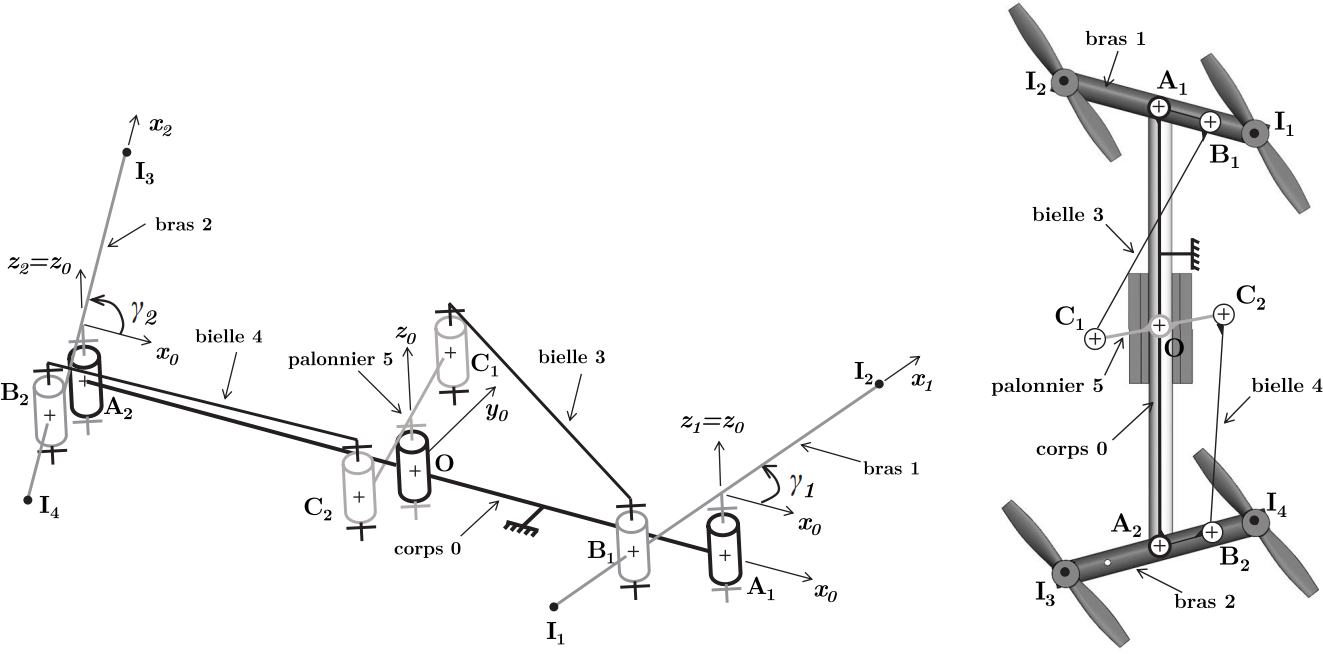
\includegraphics[width=\linewidth]{fig_10}
\caption{\label{fig:10} Modélisation cinématique en perspective et plane en vue de dessus du mécanisme de mise en mouvement des bras du drone basé sur un double système 4 barres}
\end{figure}

%%Q17
%\question{\label{q:17} Calculer le degré d’hyperstaticité de la modélisation spatiale du mécanisme de repliement. Détailler votre analyse en précisant selon la méthode retenue : le nombre
%d’équations (cinématique ou statique), le nombre d’inconnues (cinématique ou statique) et le nombre de mobilités (utile et interne) en expliquant à quel(s) mouvement(s)
%et à quelle(s) pièce(s) ces mobilités sont associées.}
%\ifprof
%\begin{corrige}
%\end{corrige}
%\else
%\fi

Une telle hyperstaticité impose des contraintes géométriques de position et d’orientation des
liaisons afin d’assurer l’assemblage du mécanisme.

%%Q18
%\question{\label{q:18} Préciser succinctement quelle(s) contrainte(s) géométrique(s) est(sont) à respecter
%pour assurer l’assemblage de ce mécanisme ?}
%\ifprof
%\begin{corrige}
%\end{corrige}
%\else
%\fi

%%Q19
%\question{\label{q:19} En modifiant la nature de certaine(s) liaison(s), proposer un modèle de mécanisme de
%repliement isostatique basé sur un double système 4 barres.
%Justifier votre proposition en reprenant le calcul du degré d’hyperstaticité.}
%\ifprof
%\begin{corrige}
%\end{corrige}
%\else
%\fi

Pour limiter les contraintes géométriques liées au mécanisme 4 barres et afin de réduire
encore le poids, le mécanisme précédent a été modifié par un mécanisme à câbles piloté
par un servomoteur (\autoref{fig:11}). De plus, du fait de la dimension des bielles et des liaisons
avec les bras, le mécanisme 4 barres ne permettait pas l’alignement complet des bras le
long du corps (position $\gamma_1 = 0\degres$), ce qu’autorise désormais le mécanisme à câbles.

\begin{figure}[H]
\centering
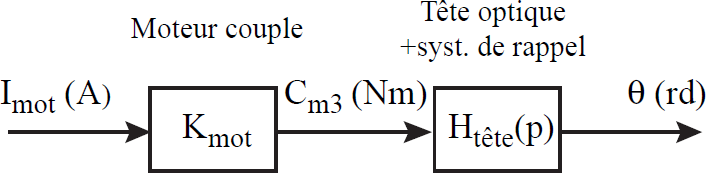
\includegraphics[width=.8\linewidth]{fig_11}
\caption{\label{fig:11} Mécanisme de repliement avec servomoteur, poulie, 2 câbles métalliques et un
élastique.}
\end{figure}

Ce mécanisme à câbles permet de réduire la masse du mécanisme de repliement à 6\% de
la masse totale du drone (exigence Id 1.1.2). Le servomoteur est placé au centre du drone
et permet de positionner les bras à l’angle désiré. La transmission du mouvement se fait
grâce aux deux câbles métalliques. 

Selon la \autoref{fig:25} de l’annexe 4, le câble métallique \textbf{1}
est accroché d’un côté à la poulie, elle­-même liée à l’axe du servomoteur, et de l’autre côté
au bras \textbf{1} au point $B_1$; 
le câble métallique 2 est accroché d’un côté à la poulie et de l’autre
au bras \textbf{2} au point $B_2$.


Afin de verrouiller la structure pour n’importe quelle position des bras, un élastique relie les
bras entre eux. Cet élastique est fixé aux bras du côté opposé aux points d’accroche des
câbles métalliques et est guidé par l’intermédiaire d’une gorge au niveau de la poulie. La
tension de l’élastique est ajustée afin de trouver un bon compromis entre le temps de repliement/dépliement des bras et la rigidité de la structure (c’est­à­dire l’absence de mouvement
des bras durant le vol en position $\gamma_1 = 90\degres$).

L’étude suivante porte sur l’analyse de la loi entrée / sorties de ce mécanisme de repliement
des bras présenté en \autoref{fig:25} de l’annexe 4. La loi entrée / sorties correspond à la relation
entre la rotation du servomoteur et les rotations des bras du drone. L’analyse va permettre
de déterminer la course angulaire à donner au servomoteur pour passer de la position bras
dépliés ($\gamma_1 = 90\degres$) à la position bras alignés ($\gamma_1 = 0\degres$), mais également les dimensions géométriques nécessaires au bon fonctionnement du mécanisme. Le paramétrage nécessaire
à cette étude est donné en annexe 4.

\begin{hypo}
\begin{itemize}
\item On suppose les câbles métalliques suffisamment rigides pour pouvoir être considérés
inextensibles en traction, compte tenu d’une part des efforts nécessaires pour mettre
en mouvement les bras et d’autre part de l’action de l’élastique.
­\item Les câbles s’enroulent sur la poulie sans glisser.
\item On considère le câble non enroulé sur la poulie entre les points $C_1$ et $B_1$. Mais en réalité
il l’est sur une faible portion et en toute rigueur $C_1B_1$ ne peut être considéré rectiligne.
Cette approximation permet de simplifier la géométrie du mécanisme et n’engendre
pas de grandes différences sur la valeur de la longueur du câble entre les points $C_1$ et
$B_1$.
\end{itemize}
\end{hypo}


%Q20
\question{\label{q:20} À partir du paramétrage et des hypothèses retenues, écrire la fermeture vectorielle
liée à la chaîne de solides \{corps 0, bras 1, câble 1 et poulie 5\}.
La mettre sous la forme $L_{c1}(\theta) \vx{1} = ...$.}
\ifprof
\begin{corrige}
\end{corrige}
\else
\fi

%Q21
\question{\label{q:21} En déduire une relation du type : $L_{c1}^2 = A\cos\gamma_1 + B\sin\gamma_1 + C$.
Exprimer les constantes $A$, $B$ et $C$ en fonction des données géométriques.}
\ifprof
\begin{corrige}
\end{corrige}
\else
\fi

Si besoin, on donne pour la suite : $A = -\SI{11200}{mm^2}$, 
$B = \SI{2400}{mm^2}$ et 
$C = \SI{22100}{mm^2}$.

%Q22
\question{\label{q:22} Déterminer approximativement la valeur numérique de $L_{c1}^{\text{init}}$
obtenue pour $\gamma_1 = 90\degres$ et $\theta=0\degres$.
Déterminer approximativement la valeur numérique de $L_{c1}^{\text{final}}$ obtenue pour $\gamma_1 = 0\degres$ et $\theta=\Delta\theta$.
En déduire la valeur approchée en degrés de la course angulaire $\Delta\theta$ nécessaire pour
assurer le repliement du bras 1, lorsque $\gamma_1$ passe de 90\degres à 0\degres.}
\ifprof
\begin{corrige}
\end{corrige}
\else
\fi


Avec la géométrie retenue et les positions des points d’accroche des câbles métalliques sur
les bras, il est nécessaire que le câble métallique \textbf{2} soit enroulé sur la poulie avec un rayon
d’enroulement $R_2$ différent de $R_1$ pour assurer que le bras \textbf{2} tourne bien de 90\degres lorsque la
poulie tourne de $\Delta \theta$. La fermeture vectorielle de la chaîne de solides corps \textbf{0}, bras \textbf{2}, câble \textbf{2}
et poulie \textbf{5} permet d’obtenir le système de deux équations suivantes pour lesquelles $R_2$ et
$L_{c2}^{\text{final}}$ restent inconnues :
$$
\left\{
\begin{array}{l}
\left(L_{c2}^{\text{init}}\right)^2 = \left(a_2 -R_2\right)^2 + \left(\dfrac{L_0}{2}\right)^2 \\
\left(L_{c2}^{\text{init}} + R_2 \Delta \theta \right)^2 = \left(\dfrac{L_0}{2} + a_2\right)^2 + R_2^2
\end{array}
\right. .
$$


En reliant ces deux équations à l’aide du terme $L_{c2}^{\text{init}}$, on montre que $R_2$ vérifie une équation
du type $f(R_2) = 0$. La \autoref{fig_12} donne l’évolution de $f(R_2)$ pour $R_2 \in \left [\SI{10}{mm}, \SI{40}{ mm}\right]$.


\begin{figure}[H]
\centering
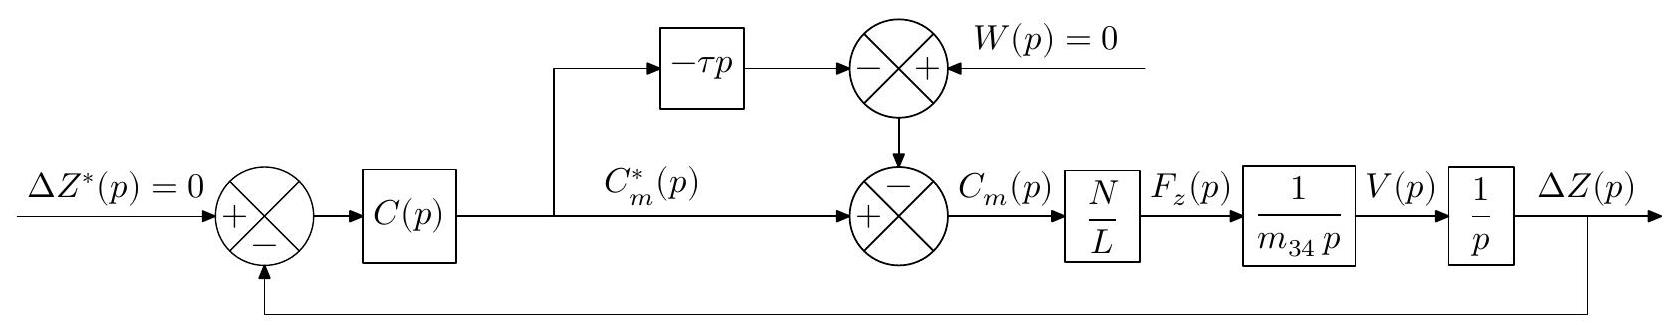
\includegraphics[width=.8\linewidth]{fig_12}
\caption{\label{fig:12} Évolution de $f(R_2)$}
\end{figure}

%Q23
\question{\label{q:23}Déterminer à l’aide de la courbe de la \autoref{fig:12} une valeur approchée de $R_2$ solution
du système d'équation précédent. La valeur numérique de $L_{c2}^{\text{init}}$ correspondante est alors $L_{c2}^{\text{init}} \simeq \SI{141}{mm}$. }
\ifprof
\begin{corrige}
\end{corrige}
\else
\fi

Des essais à vide (hélices et drone à l’arrêt) ont été réalisés pour l’étude des performances
du système de repliement/dépliement avec les dimensions déterminées précédemment. Les
résultats de ces essais sont donnés en \autoref{fig:13} pour la phase de repliement et en \autoref{fig:14}
pour la phase de dépliement. Sur ces courbes, le trait fort représente la valeur moyenne des
positions angulaires des différents essais

%Q24
\question{\label{q:24} Les critères de performance de l’exigence Id 1.1.2 liés au mécanisme de repliement/­
dépliement sont­ils respectés ?}
\ifprof
\begin{corrige}
\end{corrige}
\else
\fi

%Q25
\question{\label{q:25} Expliquer l’origine physique des oscillations observées sur la position angulaire du
bras \textbf{1} et dans une moindre mesure sur la position angulaire du bras \textbf{2} lors du dépliement des bras.}
\ifprof
\begin{corrige}
\end{corrige}
\else
\fi

\section{\label{sec:03} Analyse simplifiée de l’asservissement du drone}

La structure générale de commande du drone est constituée de différents éléments présentés de manière schématique en \autoref{fig:15}. On y retrouve :
\begin{itemize}
\item le contrôleur de position qui génère les valeurs de consigne en attitude 
(angles de roulis $\theta_R$, 
de tangage $\theta_T$ 
et de lacet $\theta_L$)
et de poussée des moteurs ;
\item­ le contrôleur d’attitude, qui permet de contrôler l’orientation du drone dans l’espace;
\item­ l’estimateur d’attitude, qui est composé de gyroscopes et accéléromètres pour estimer
les angles de roulis $\theta_R$, tangage $\theta_T$ et d’un magnétomètre afin d’obtenir le cap du drone
(angle de lacet $\theta_L$);
­ l’estimateur de position qui est composé de la caméra embarquée et d’un baromètre
afin d’estimer les positions et vitesses du drone.
\end{itemize}

\begin{obj}
L’objectif de cette partie est de vérifier que les performances de contrôle en roulis sont
conservées lors du passage de l’ouverture et lors de l’activation du mécanisme de repliement/dépliement des bras. On se limite pour cela à la structure encadrée en pointillés de la
\autoref{fig:15}.
\end{obj}

\begin{figure}[H]
\centering
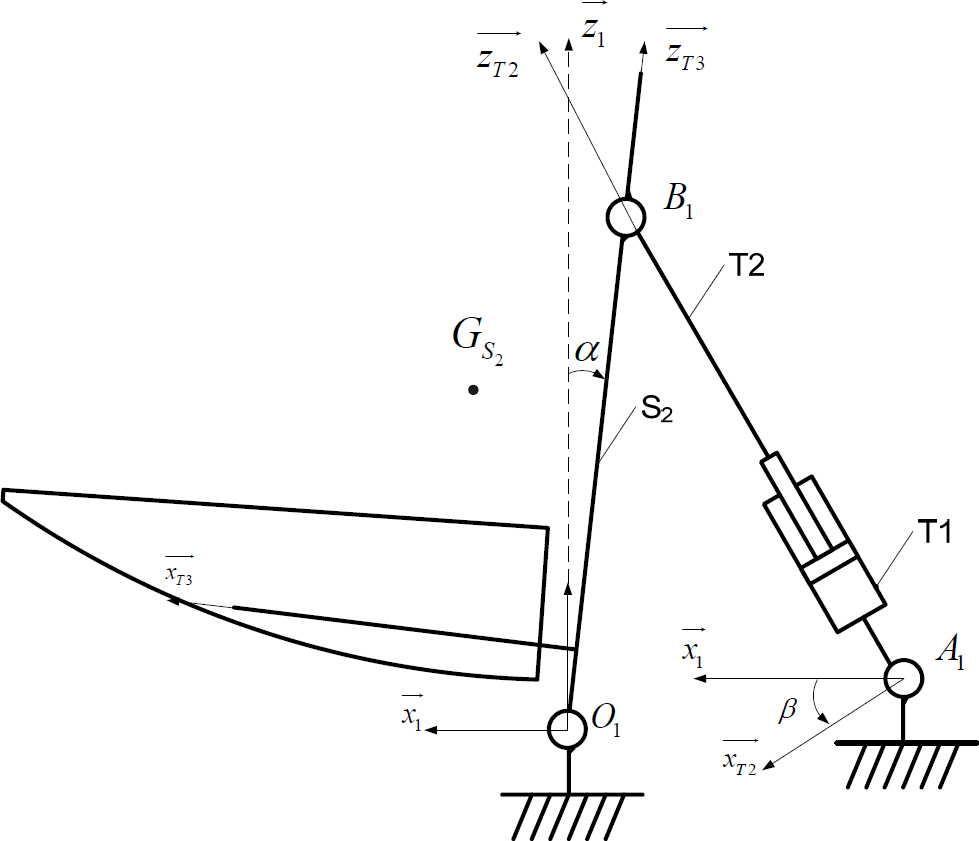
\includegraphics[width=.8\linewidth]{fig_13}
\caption{\label{fig:13} Relevés des angles $\gamma_1$ et $\gamma_2$ pour la phase de repliement}
\end{figure}

\begin{figure}[H]
\centering
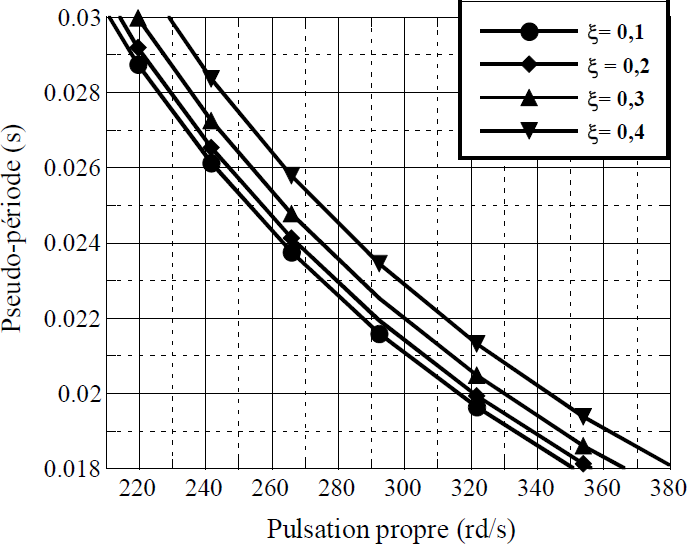
\includegraphics[width=.8\linewidth]{fig_14}
\caption{\label{fig:14} Relevés des angles $\gamma_1$ et $\gamma_2$ pour la phase de dépliement}
\end{figure}


\begin{figure}[H]
\centering
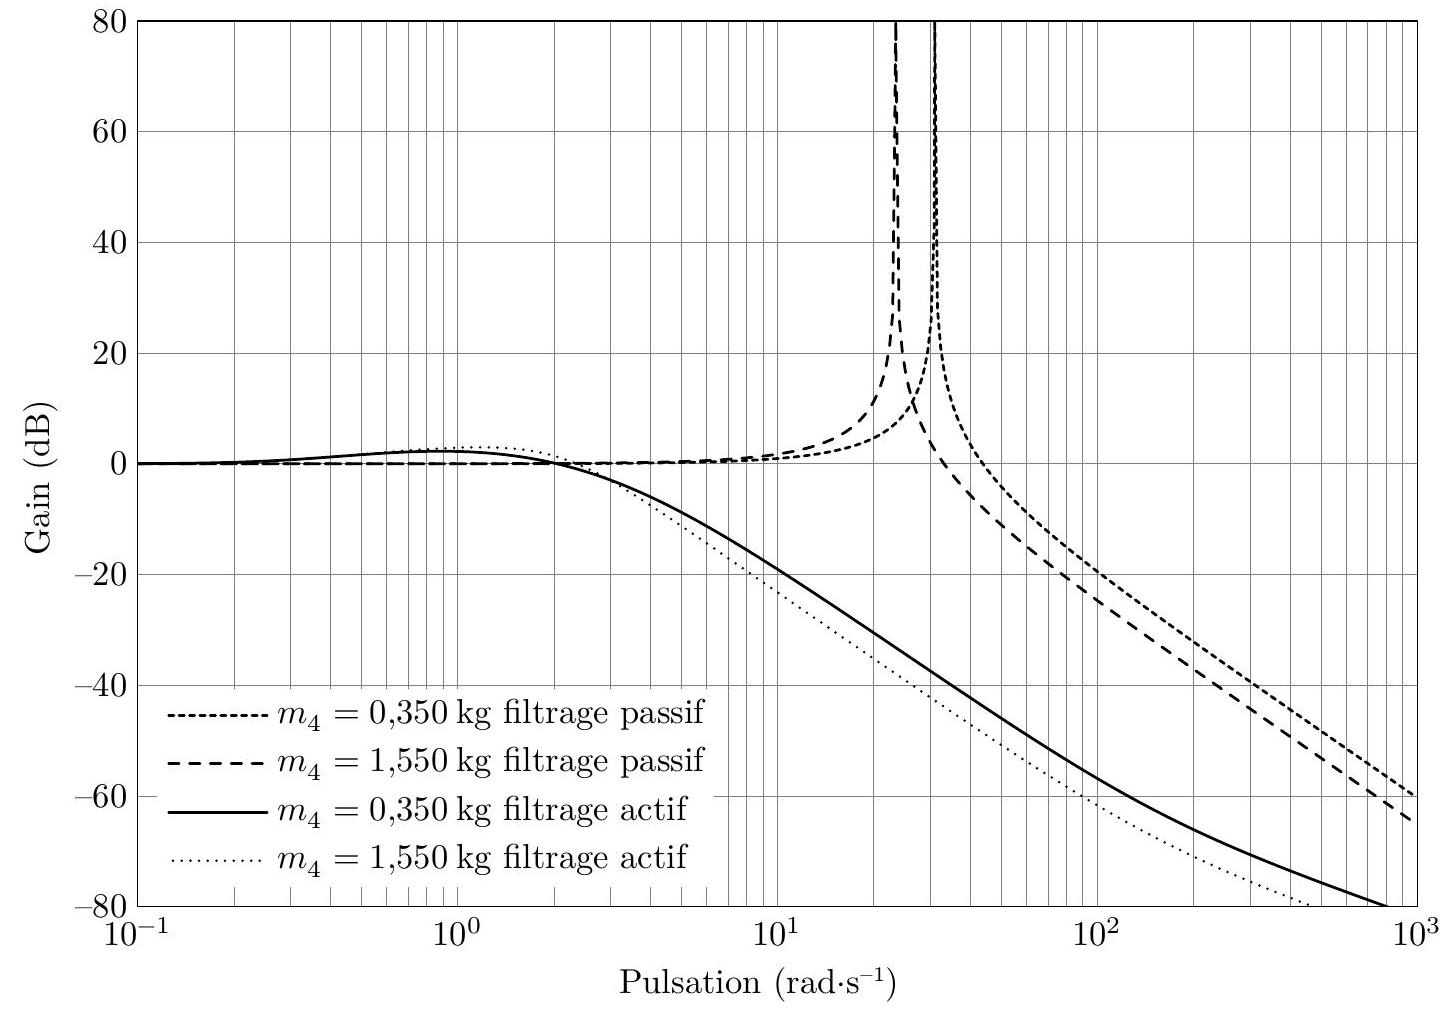
\includegraphics[width=.8\linewidth]{fig_15}
\caption{\label{fig:15} Structure de commande du drone}
\end{figure}

\subsection{­Modélisation du comportement des moteurs brushless}

Chaque hélice du drone est actionnée par un moteur brushless, lui-même alimenté par un
ESC (Electronic Speed Controller). L’ESC est un contrôleur qui permet de faire varier la
vitesse de rotation du moteur à l’aide d’une commande PPM (Pulse Position Modulation). Il
génère ainsi les signaux pour les trois phases du moteur.

En vue d’établir un modèle de comportement des moteurs brushless, la vitesse de rotation du
moteur $\omega_M(t)$ en \si{tr/min} est mesurée pour une variation $u(t)$ de type échelon de la commande
PPM de \SI{40}{\%} puis de 80\% sans unité. Cette évolution est donnée sur la figure du DR de la
question \ref{q:26}.

Suite à cet essai, on propose de modéliser le comportement du moteur brushless par celui
d’un système du premier ordre, reliant $\Omega_M(p)$ la transformée de Laplace de la vitesse de rotation à
$U(p)$ la transformée de Laplace de la commande PPM. On note $\indice{H}{mot}(p) = \dfrac{\Omega_M(p)}{
U(p)}$ la fonction de transfert du moteur.

%Q26
\question{\label{q:26} Justifier le modèle de comportement retenu pour $\indice{H}{mot}(p)$ et déterminer ses caractéristiques (valeurs numériques et unités à préciser). Faire apparaître sur la figure du DR
les tracés permettant de déterminer les caractéristiques de $\indice{H}{mot}(p)$.}
\ifprof
\begin{corrige}
\end{corrige}
\else
\fi

\subsection{Modélisation du comportement des hélices}
Afin d’obtenir un modèle fiable pour le contrôle du drone, les composantes de poussée
$T$ et de traînée $Q$ de l’action de l’air sur l’hélice sont identifiées pour le couple moteur/
hélice grâce à un banc d’essai. Ce banc d’essai, \autoref{fig:17}, est équipé de deux capteurs
d’effort $C1$ et $C2$, chacun muni de 4 jauges de déformation, et d’un capteur optique pour
mesurer la vitesse de l’hélice. On rappelle, \autoref{fig:16}, qu’un capteur d’effort avec les jauges
de déformation ainsi positionnées et orientées sur le corps d’épreuve du capteur permet
d’accéder à la valeur de l’effort $F$ appliqué sur le capteur.


%Q27
\question{\label{q:27} Justifier la nécessité de décaler l’axe de rotation du moteur de l’axe du capteur d’effort
$C1$ d’une distance $d_y$ et en déduire quel capteur d’effort $C1$ ou $C2$ permet de mesurer
quelle composante de l’action (effort de poussée $T$ ou moment de traînée $Q$).}
\ifprof
\begin{corrige}
\end{corrige}
\else
\fi

\begin{figure}[H]
\centering
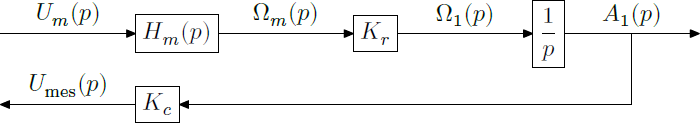
\includegraphics[width=.35\linewidth]{fig_16}
\caption{\label{fig:16} Capteur d’effort. Deux jauges visibles au dessus, les deux autres en dessous}
\end{figure}

\begin{figure}[H]
\centering
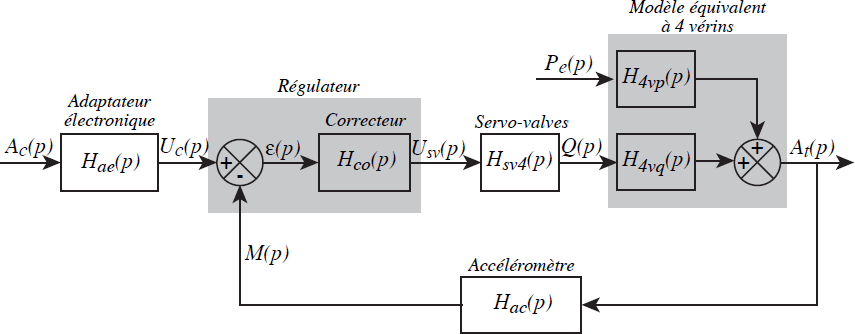
\includegraphics[width=.9\linewidth]{fig_17}
\caption{\label{fig:17} Vue et schéma du banc d’essai pour déterminer les composantes $T$ et $Q$ de
l’action de l’air sur l’hélice en fonction de la vitesse de rotation de l’hélice}
\end{figure}

Les différentes mesures permettent de déterminer les évolutions de l’effort de poussée $T$ et
du moment de traînée $Q$ en fonction de la vitesse de rotation $\omega_1$ de l’hélice. Ces évolutions
sont présentées sur les figures du DR de la question \ref{q:28}. Les mesures confirment une évolution
quadratique de $T$ et $Q$ en fonction de $\omega_1$, avec :
$T = c_T \omega_1^2$ avec $c_T = \SI{1e-6}{N/(rad/s)^2}$ et
$Q = c_Q \omega_1^2$ avec $c_Q = \SI{9.8e-6}{N/(rad/s)^2}$ 
où $c_T$ et $c_Q$, les coefficients de poussée, respectivement de traînée, sont obtenus par régression linéaire.

Afin de pouvoir modéliser le comportement de l’asservissement en roulis du drone lors du
passage de l’ouverture, il est nécessaire de proposer un modèle de comportement linéarisé
de chacun des composants du drone et notamment des hélices. On se place pour cela autour
du point de fonctionnement correspondant à la vitesse d’approche du drone de l’ouverture,
ce qui correspond à une vitesse de rotation des hélices de l’ordre de \SI{1400}{rad.s^{-1}}. On estime
que les variations de vitesse de rotation des hélices sont au maximum de $\pm \SI{500}{rad.s^{-1}}$ lors
des corrections d’attitude et de cap nécessaires au passage de l’ouverture.

%Q28
\question{\label{q:28} Proposer un modèle de comportement linéarisé de la variation de l’effort de poussée
$\Delta T$ et $\Delta Q$ en fonction de la variation de vitesse de rotation $\Delta \omega_1$ autour du point de
fonctionnement étudié ($\omega_1 \simeq \SI{1400}{rad.s^{-1}}$) et valable dans le domaine de variation de
$\pm \SI{500}{rad.s^{-1}}$ considéré. Laisser apparents sur les courbes du DR les tracés permettant de justifier votre démarche.}
\ifprof
\begin{corrige}
\end{corrige}
\else
\fi

\subsection{Analyse du contrôleur d’attitude en roulis}

Dans cette sous­partie, on s’intéresse au réglage du contrôleur d’attitude en roulis dans le
cas d’une commande en échelon sans perturbation. Puis, nous verrons comment se comporte le drone en roulis lors du passage de l’ouverture (ajout d’une perturbation) et enfin
son comportement lors du repliement des bras. L’objectif est de s’assurer que le réglage du
contrôleur d’attitude permet de conserver, dans une certaine mesure, le contrôle en roulis
lors du passage de l’ouverture et lors du repliement/dépliement des bras.

\begin{figure}[H]
\centering
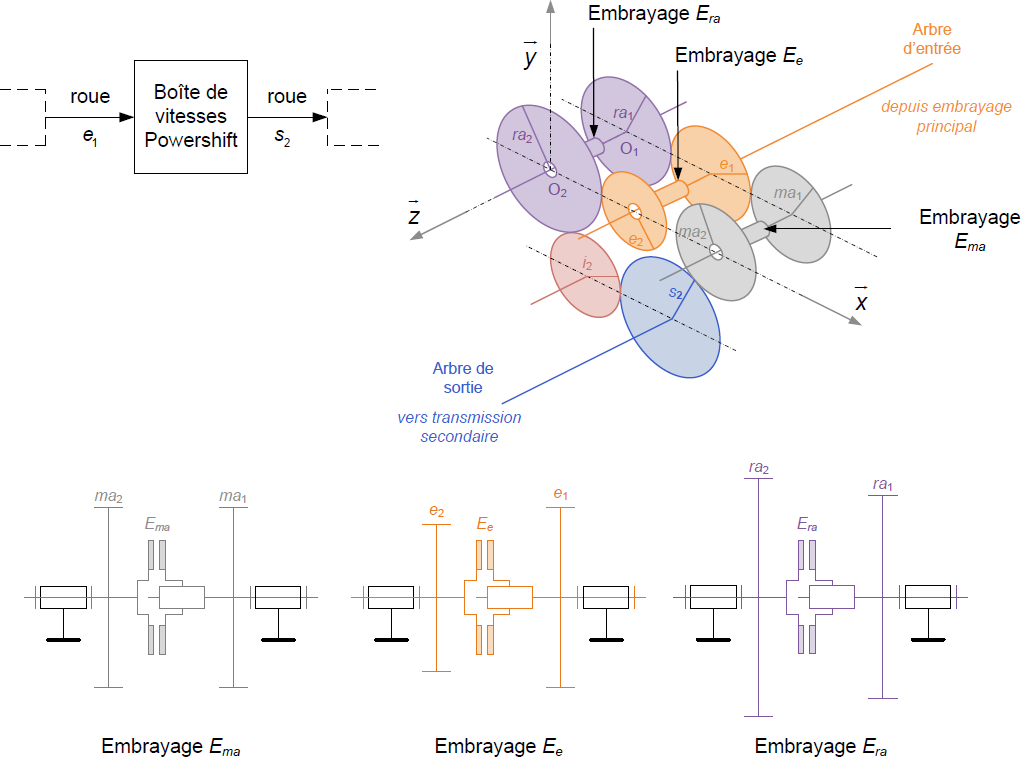
\includegraphics[width=.8\linewidth]{fig_18}
\caption{\label{fig:18} ­ Représentation simplifiée par schéma-blocs de l’asservissement du drone en
roulis, angle $\theta_R$ en degrés}
\end{figure}

L’asservissement du drone en roulis, angle $\theta_R$, est représenté par le schéma bloc de la
\autoref{fig:18}. Les performances de cet asservissement sont décrites par l’exigence Id 2 du
diagramme des exigences donné en \autoref{fig:21} annexe 1. Les grandeurs indiquées sur le
schéma bloc de la \autoref{fig:18} représentent les transformées de Laplace des grandeurs obtenues pour des variations autour du point de fonctionnement $\theta_R = 0\degres$. La vitesse de rotation du
drone en roulis en \si{deg/s} est notée $\Omega_R(p)$. Le contrôleur d’attitude est un correcteur de fonction de transfert $C(p)$ de sortie $U(p)$ en incréments (inc). Le comportement de l’estimateur
d’angle en roulis (composé d’un gyromètre, d’un accéléromètre et d’un système de traitement des signaux) est modélisé par un gain pur $K_E$, tel que $K_E = \SI{150}{inc/deg}$.
Le bloc adaptateur, de gain pur $K_A = K_E$, permet d’adapter la consigne de variation d’angle
de roulis $\theta_R^C(p)$ en degrés en une grandeur comparable à la mesure de l’estimateur d’angle
de roulis.
La fonction de transfert $H_S (p) = \dfrac{\Omega_R(p)}{U(p)}$ représente le comportement linéarisé autour d’un
point de fonctionnement (vol d’approche à vitesse constante) du drone dans la position bras
déplié $\gamma_1 = 90\degres$. Ce comportement a été défini, entre autres, à partir des résultats des analyses des parties précédentes.


Une simulation a permis de tracer les diagrammes de Bode de la réponse fréquentielle de
$H_S (p)$. Cette réponse est donnée sur la figure du DR de la question \ref{q:29}, où l’on retrouve l’évolution du
gain $G_{HS}(\omega) = 20 \log |H_S (j\omega)|$ et de la phase $\Phi_{HS} (\omega) = \arg\left(H_S (j\omega)\right)$ en fonction de la pulsation $\omega$.

Compte tenu de la réponse fréquentielle de $H_S (p)$, on propose le modèle suivant pour $H_S (p)$ :
$H_S(p)=\dfrac{K_S}{1+\dfrac{2z_S}{\omega_{0S}}p+\dfrac{1}{\omega_{0S}^2}p^2}$.


%Q29
\question{\label{q:29} Justifier le choix retenu pour l’expression de $H_S (p)$ et déterminer graphiquement les
valeurs numériques et unités des paramètres caractéristiques $K_S$ , $z_S$ et $\omega_{0S}$ . Faire apparaître sur la figure du DR, les constructions permettant de justifier les valeurs proposées.}
\ifprof
\begin{corrige}
\end{corrige}
\else
\fi


%Q30
\question{\label{q:30} Tracer, sur la figure du DR, les courbes de gain $\indice{G}{BO}(\omega)$ et de phase $\indice{\Phi}{BO}(\omega)$ de la réponse fréquentielle de la fonction de transfert en boucle ouverte $\indice{H}{BO}(p) = \dfrac{\theta_{R}^{\text{mes}}(p)}{\varepsilon(p)}$
non corrigée, c’est-à-dire pour $C(p) = 1$. Justifier vos tracés.}
\ifprof
\begin{corrige}
\end{corrige}
\else
\fi

%Q31
\question{\label{q:31}  Représenter, sur le DR, les marges de gain $MG$ et marge de phase $M\Phi$ de la FTBO si
elles sont définies. Conclure sur les performances de l’asservissement en roulis sans
correction (exigence Id 2).}
\ifprof
\begin{corrige}
\end{corrige}
\else
\fi

On s’intéresse tout d’abord à l’effet de l’action proportionnelle du contrôleur d’attitude et on
pose $C(p) = K_P$.


%Q32
\question{\label{q:32} Déterminer graphiquement la valeur à donner à $K_P$ pour vérifier le critère de stabilité.}
\ifprof
\begin{corrige}
\end{corrige}
\else
\fi


D’après les résultats des simulations, l’action proportionnelle du contrôleur d’attitude permettrait le respect des performances en roulis dans le cas de vol non perturbé. La prise en
compte des perturbations est complexe à modéliser sur un tel système, aussi on considère
en première approximation que les perturbations en vol contribuent à une variation de vitesse
de roulis $P(p)$, modélisée par la suite comme une perturbation de type échelon d’amplitude $P_0$
(\autoref{fig:19}).

\begin{figure}[H]
\centering
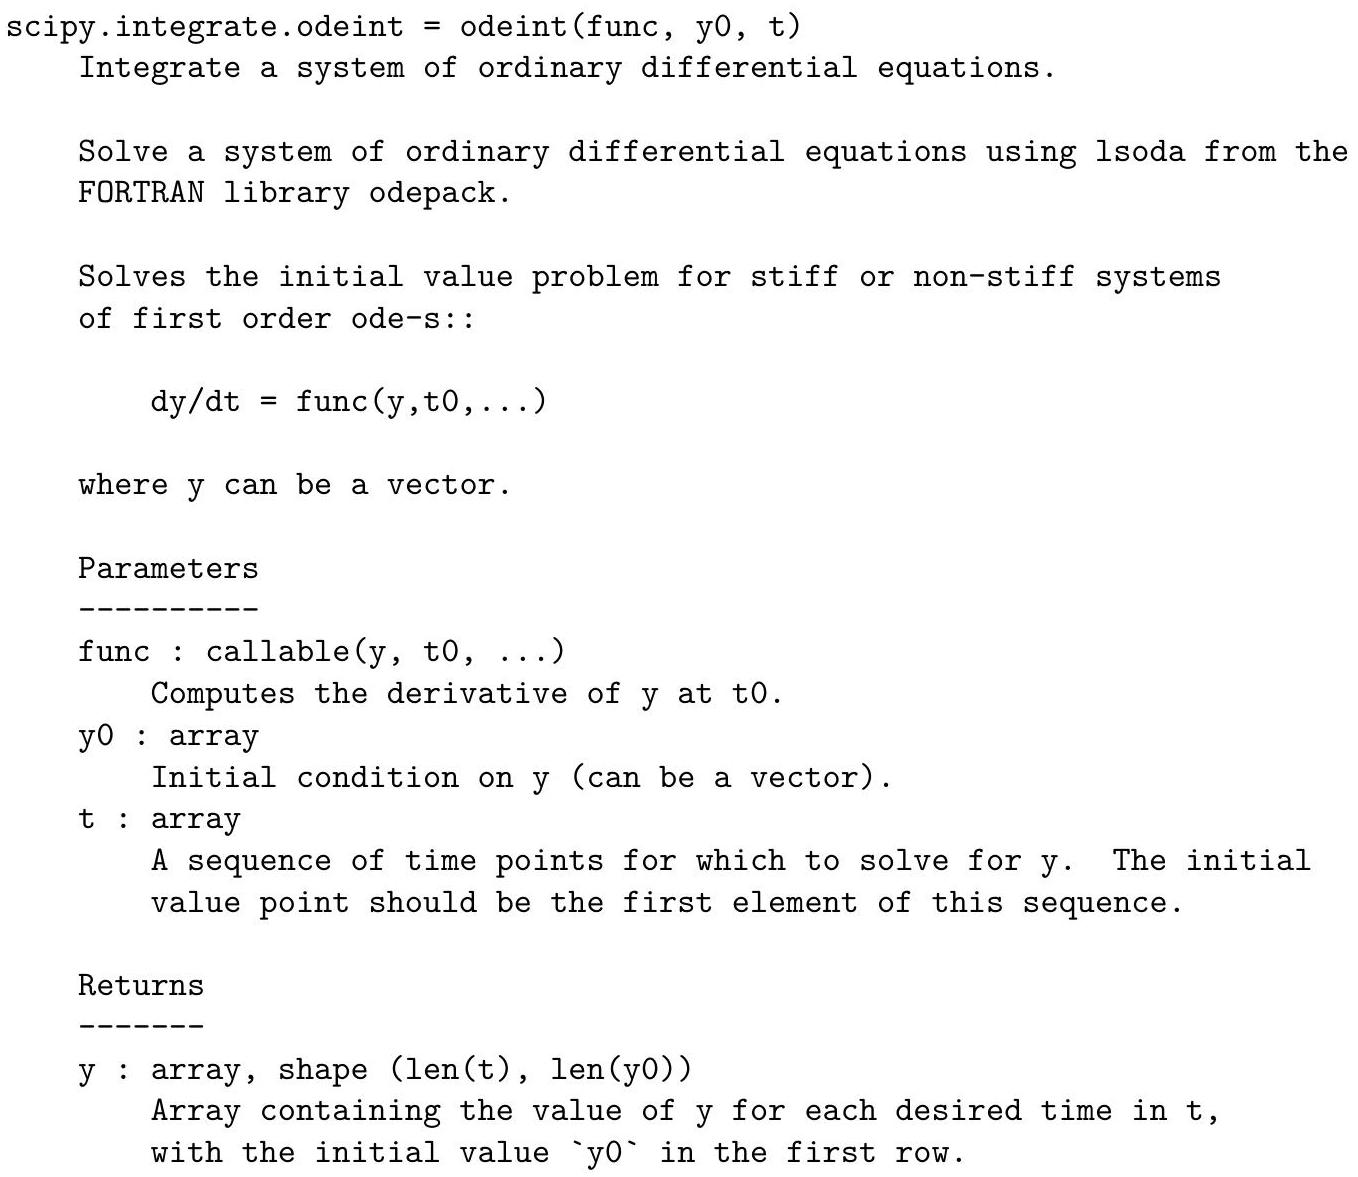
\includegraphics[width=.8\linewidth]{fig_19}
\caption{\label{fig:19} Représentation par schéma bloc avec prise en compte des perturbations en vol}
\end{figure}


%Q33
\question{\label{q:33} Déterminer l’expression de $\theta_R(p)$ en fonction de $\theta_R^C(p)$
 et de $P(p)$. On rappelle que $C(p) = K_P$ et $H_S (p)$ est définie par l’équation (2).}
\ifprof
\begin{corrige}
\end{corrige}
\else
\fi

%Q34
\question{\label{q:34} Déterminer l’expression de la contribution de la perturbation de type échelon d’amplitude $P_0$ sur la valeur de $\theta_R(t)$ en régime établi dans le cas où la consigne est nulle $\theta_R^C(t)=0\degres$.}
\ifprof
\begin{corrige}
\end{corrige}
\else
\fi

%Q35
\question{\label{q:35} Quelle valeur donner à $K_P$ pour respecter le critère de précision vis-­à-­vis de la perturbation ? Conclure sur les limites de la correction proportionnelle.}
\ifprof
\begin{corrige}
\end{corrige}
\else
\fi

Il est alors décidé de mettre en place une correction proportionnelle intégrale (correcteur PI)
avec $C(p) = K_P\left(\dfrac{1+T_i p}{T_i p}\right)$. On fixe pour la suite $K_P = 0,1$.

%Q36
\question{\label{q:36} Justifier que cette correction permet de satisfaire les critères de précision sur la
consigne et sur la perturbation.}
\ifprof
\begin{corrige}
\end{corrige}
\else
\fi

Les figures du DR de la question \ref{q:37} donnent les résultats de la simulation du système avec la
correction proportionnelle intégrale retenue. La première donne l’évolution de $\theta_R(t)$ pour une
consigne de roulis $\theta_R^C(t)$ de type échelon d’amplitude $\theta_{R0}^C = 10\degres$ et pour une perturbation $P(t)$ de
type échelon d’amplitude $P_0 =\SI{10}{deg/s}$ appliquée en $t = \SI{2}{s}$. La seconde donne les courbes
de gain et de phase du diagramme de Bode de la réponse fréquentielle de la FTBO corrigée.

%Q37
\question{\label{q:37} Vérifier les performances temporelles et déterminer les marges de gain et de phase
de la FTBO avec correction. Faire apparaître les constructions sur les figures du DR.
Conclure sur le réglage et le choix d’un correcteur PI.}
\ifprof
\begin{corrige}
\end{corrige}
\else
\fi

Des essais en vol ont été réalisés avec le réglage précédent pour la partie roulis du contrôleur
d’attitude. Ces essais décrivent le comportement en roulis du drone lors du repliement des
bras, du passage de l’ouverture et du dépliement des bras. Les évolutions de l’angle de
roulis (en degrés) et de la vitesse de rotation en roulis (en \si{deg/s}) du drone sont données
en figure 20 pour 10 essais. Sur cette figure, l’origine des temps, $t = \SI{0}{s}$, correspond au
déclenchement de la procédure de repliement des bras, l’ouverture est traversée par le drone
à partir de l’instant $t = \SI{0,25}{s}$ jusqu’à $t = \SI{0,5}{s}$ et le dépliement des bras débute pour $t = \SI{0,5}{s}$.

\begin{figure}[H]
\centering
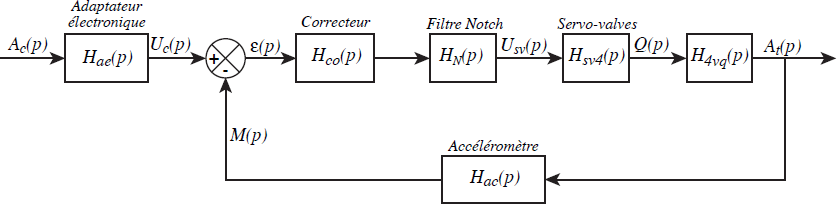
\includegraphics[width=.8\linewidth]{fig_20}
\caption{\label{fig:20} ­Évolutions de l’angle de roulis (en degrés) et de la vitesse de rotation en roulis
(en \si{deg/s}) du drone sont donnée pour 10 essais.}
\end{figure}

%Q38
\question{\label{q:38} Conclure sur l’influence de la phase de repliement des bras et du passage de l’ouverture sur le comportement en roulis du drone avec la correction retenue.}
\ifprof
\begin{corrige}
\end{corrige}
\else
\fi


\newpage

\section*{Annexe 1}


\begin{figure}[H]
\centering
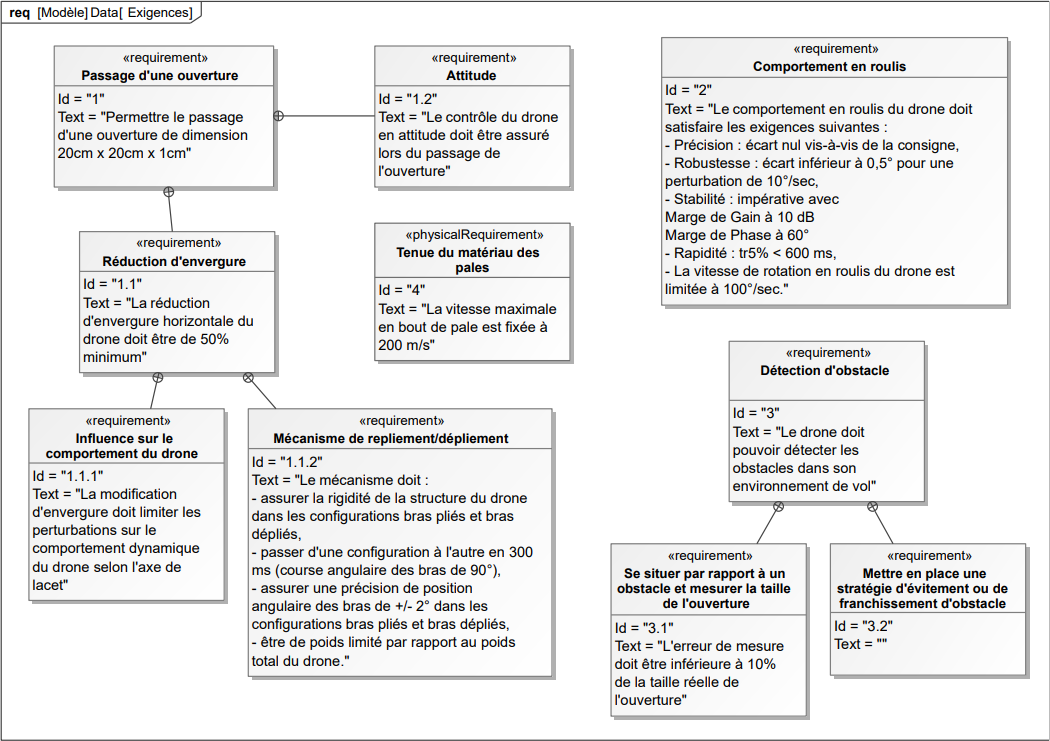
\includegraphics[width=\linewidth]{fig_21}
\caption{\label{fig:21} Diagramme partiel des exigences liées au passage de l’ouverture de la plateforme QuadMorphing}
\end{figure}

\begin{figure}[H]
\centering
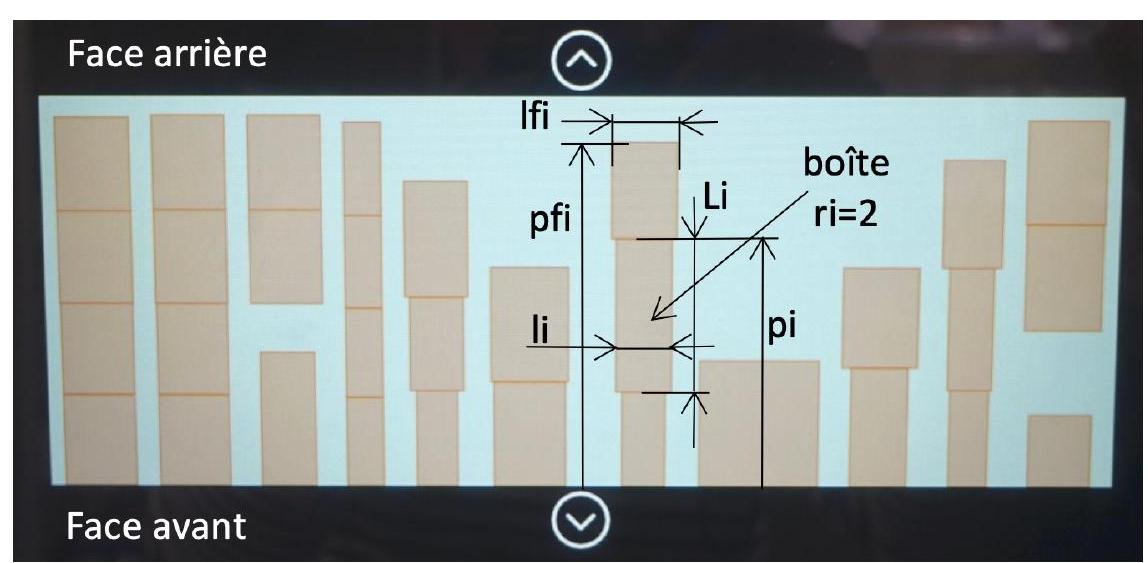
\includegraphics[width=\linewidth]{fig_22}
\caption{\label{fig:22} Diagramme de définition des blocs de la plateforme QuadMorphing}
\end{figure}

\newpage

\section*{Annexe 2}
\textbf{Notations}

La base $\bas{0}$ associée au repère $\rep{0}$ est notée $\repere{O}{x_0}{y_0}{z_0}$. Il en est de même pour le repère $\rep{1}$ associé au bras 1 et pour le repère $\rep{H1}$ associé à l’hélice $H1$. On note :
\begin{itemize}
\item $\ell$ et $L$, respectivement la largeur et la longueur du parallélépipède rectangle englobant
la totalité du drone (représenté en pointillés sur la \autoref{fig:23}), de hauteur $h = \SI{115}{mm}$,
constante quelle que soit la configuration du drone;
\item $L_0 = \SI{280}{mm}$, la longueur du corps 0;
\item $\vect{­OA_1} = \dfrac{L_0}{2} \vx{0} + \dfrac{h}{4}\vz{0}$;
\item $L_1 = \SI{140}{mm}$, la longueur du bras 1;
\item $\vect{I_1A_1} = \dfrac{L_1}{2} \vx{1} - \dfrac{h}{4} \vz{0}$;
\item $r_h = \SI{64}{mm}$, la longueur d’une pale de l’hélice;
\item $\vect{I_1 P} = r_h \vect{x_{H1}}$ pour l’hélice H1.
\end{itemize}

\begin{figure}[H]
\centering
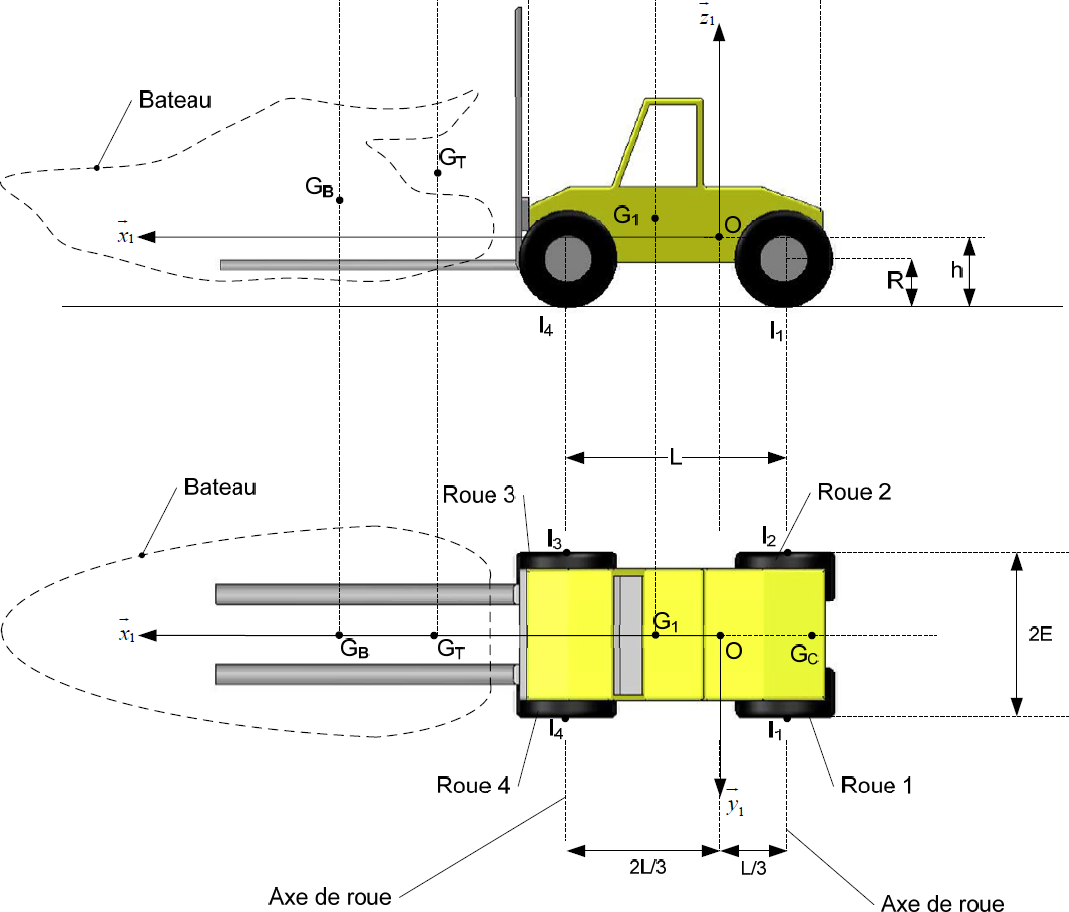
\includegraphics[width=\linewidth]{fig_23}
\caption{\label{fig:23}  Vue de dessus et en perspective du drone en phase de repliement et paramétrage de la géométrie}
\end{figure}


\begin{figure}[H]
\centering
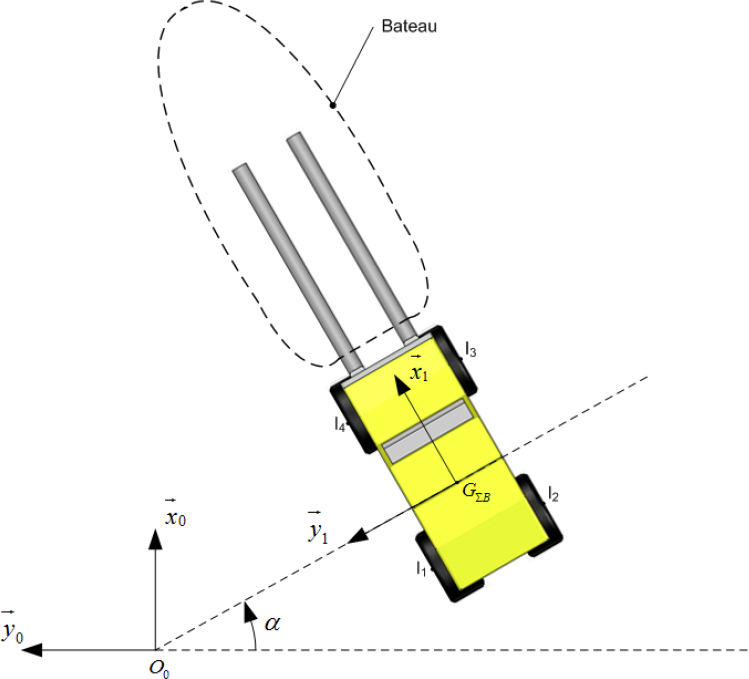
\includegraphics[width=.5\linewidth]{fig_24}
\caption{\label{fig:24} ­ Figures planes du paramétrage du bras $i$ par rapport au corps 0 du drone et de
l’hélice $H1$ par rapport au bras 1 du drone}
\end{figure}



\section*{Annexe 3}

Les matrices d’inerties des principaux éléments du drone, dont la géométrie a été simplifiée
pour cette étude, sont données ci­dessous, chacune dans la base principale d’inertie :

Pour le corps 0, de centre d’inertie O et de masse $m_c$ : $\inertie{0}{O} = \matinertie{I_{cx}}{I_{cy}}{I_{cz}}{0}{0}{0}{O,\bas{0}}$.

Pour le bras 1, de centre d’inertie $A_1$ et de masse $m_b$ : $\inertie{1}{A_1} = \matinertie{I_{bx}}{I_{by}}{I_{bz}}{0}{0}{0}{A_1,\bas{1}}$.

Pour le bras 2, de centre d’inertie $A_2$ et de masse $m_b$ : $\inertie{2}{A_2} = \matinertie{I_{bx}}{I_{by}}{I_{bz}}{0}{0}{0}{A_2,\bas{2}}$.

Pour chaque hélice $H_i (i = 1 à 4)$, de centre d’inertie $I_i$ et de masse $m_h$, le moment d’inertie
selon l’axe $\axe{I_i}{z_0}$ est noté $I_{hz}$.

On note $\Sigma$ l’ensemble constitué des principaux éléments du drone, tel que $\Sigma = \left\{ 0+1+2+\sum_{i=1}^{4}H_i \right\}$.



\section*{Annexe 4}


\begin{figure}[H]
\centering
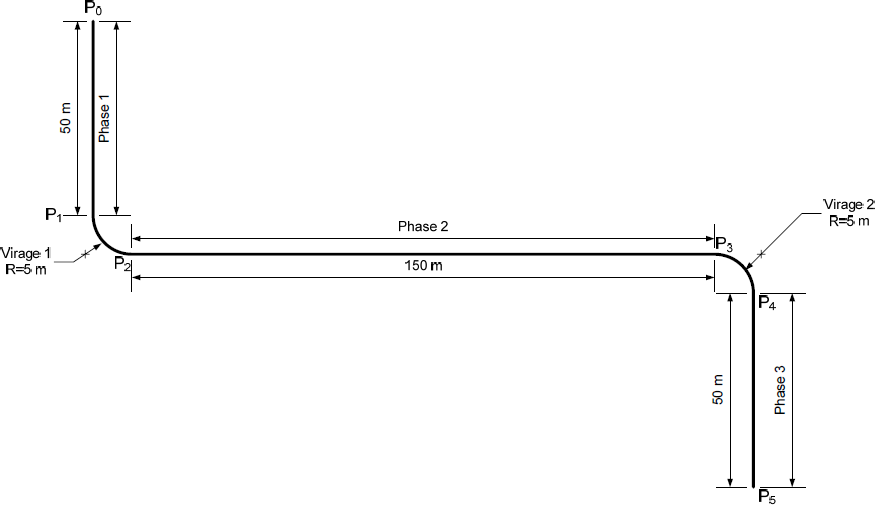
\includegraphics[width=.4\linewidth]{fig_25}
\caption{\label{fig:25} Mécanisme de mise en mouvement du bras}
\end{figure}

\textbf{Notations}
\begin{itemize}
\item l’orientation de la poulie 5 par rapport au corps du drone 0 est paramétrée par l’angle
$\theta(t)$ tel que : $\theta(t)(t) = \left(\vx{0},\vx{5}\right) = \left(\vy{0},\vy{5}\right)$;
\item­ le rayon d’enroulement du câble métallique 1 sur la poulie 5 est noté $R_1$, avec
$R_1 = \SI{30}{mm}$. Ce rayon d’enroulement correspond à la distance $OC_1$, tel que $\vect{OC_1}= R_1\vy{0}$;
\item­ en première approximation et afin de simplifier la géométrie pour l’étude de la loi entrée
/ sortie de ce mécanisme, on considère la longueur $B_1C_1$ telle que $\vect{C_1B_1} = L_{c1}(\theta) \vect{x_{c1}}$, avec $L_{c1}(\theta) = L^{\text{init}}_{c1} - R_1\theta$. La grandeur $L^{\text{init}}_{c1}$ correspond à la distance $B_1C_1$ pour $\gamma_1 = 90\degres$, on a
alors le point $P_1$ confondu avec $C_1$ et $\theta = 0\degres$;
\item­ la distance du point d’accroche $B_1$ du câble métallique 1 sur le bras 1 est notée $a_1$ telle
que $\vect{A_1B_1} = -a_1 \vx{1}$, avec $a_1 = \SI{40}{mm}$;
\item­ la distance du point d’accroche $B_2$ du câble métallique 2 sur le bras 2 est notée $a_2$ telle
que $\vect{A_2B_2} = a_2 \vect{x_2}$, avec $a_2 = a_1 = \SI{40}{mm}$;
\item­ on rappelle que $\vect{OA_1} = \dfrac{L_0}{2}\vx{0}$  avec $L_0 = \SI{280}{mm}$.
\end{itemize}

On considère la position initiale du mécanisme, en configuration bras dépliés, telle que
$\gamma_1= 90\degres$ et $\gamma_2 = 90\degres$ et donc $\theta = 0\degres$. On a alors $L_{c1}(\theta = 0\degres) = L^{\text{init}}_{c1}$ et $L_{c2}(\theta = 0\degres) = L^{\text{init}}_{c2}$.

La position finale du mécanisme est la position pour laquelle les bras sont alignés avec la
direction prépondérante du drone, c’est­à-dire pour $\vx{1} = \vx{0}$ et $\vx{2} = -\vx{0}$. On a alors $\gamma_1 = 0\degres$, $\gamma_2 = 180\degres$ et $\theta = \Delta \theta$, où $\Delta \theta$ est la course angulaire de la poulie avec $L_{c1}(\Delta \theta) = L^{\text{final}}_{c1}$ et
$L_{c2}(\Delta \theta) = L^{\text{final}}_{c2}$.